%
% Modelo para relatório de trabahlo final das disciplinas de Projecto dos
% mestrados do DI:
% - Engenharia Informática
% - Informática
% - Segurança Informática
% - Ciência de Dados
%
% Incorpora elementos impostos pelo Regulamento de Estudos Pos-Graduados da
% Universidade de Lisboa
%(Deliberacao 1506/2006 - Diario da República, 2.a série - n.o 209 -
% 30 de Outubro de 2006)
%
% Versão Setembro 2024 
%
% Algumas  dicas:
%  - Na pasta ./tex deverão estar os vários ficheiros latex que constituem o relatório
%  - Primeiro os ficheiros:
%		- capa.tex
%		- agradecimentos.tex
%		- resumo_pt.tex
%		- resumo_ing.tex
%		- No início de cada um destes ficheiros é mencionado o que é necessário/possível alterar
%  - Depois vêm os ficheiros com os capítulos, organizados da forma que entenderem e incluídos de forma apropriada no local indicado neste ficheiro main.
%  - Na pasta ./pic deverão ser colocadas as figuras
%  - A bibliografia deverá estar num ficheirona mesma directoria que este main.tex	
%
%%%%%%%%%%%%%%%%%%%%%%%%%%%%%%%%%%%%%%%%%%%%%%%%%%%%%%%%%%%%%%%%%%%%%%
\documentclass[11pt,openright,twoside]{report}

\usepackage[utf8]{inputenc}
% Quem tiver problemas com os acentos, trocar utf8 por latin1

\usepackage[english]{babel}
\usepackage{times}
\usepackage{minted}
\usepackage{placeins}
\usepackage{float}
\floatstyle{plain}
\newfloat{listing}{H}{lop}
\floatname{listing}{Listing}
\usepackage[most]{tcolorbox}
\usepackage{xcolor}

\tcbuselibrary{listings, breakable}

\usepackage{array}
\usepackage{booktabs}
\usepackage{colortbl}

% Isto é só para gerar o texto dummy do exemplo. Remover da tese.
%\usepackage{blindtext}

\usepackage{graphicx}

% Indice remissivo
\usepackage{makeidx}
\makeindex

% Glossario
\usepackage{glossaries}
\makeglossaries

% Links
\usepackage{hyperref}

% Package para cabecalhos
\usepackage{fancyhdr}
\usepackage{lastpage}

\fancyhf{} %
\lhead{\nouppercase {\leftmark}} %
\rhead{\nouppercase {\bf \thepage}}
\renewcommand{\headrulewidth}{0.1pt}

% Comando para inserir pagina em branco (inserida na numeracao, mas sem
% numero impresso) para quando e' preciso obrigar um capitulo a comecar
% do lado direito (pagina impar)
\newcommand{\LIMPA}{
\newpage
\mbox{}
\thispagestyle{empty}
}

% Igual, mas insere pagina com numero impresso (normalmente nao se usa)
\newcommand{\LIMPAC}{
\newpage
\mbox{}
\thispagestyle{plain}
}

%
% ALTERAR AQUI AS INFORMACOES RELATIVAS AO PROJECTO
%
\newcommand{\TITULO}{Título do Trabalho}
\newcommand{\Autor}{Nome Completo do Aluno}

%Orientador e CoOrientador *sem* titulos (e.g. Prof. Doutor)
\newcommand{\Orientador}{Nome Completo do Orientador}
\newcommand{\PCoOrientador}{Nome Completo do Orientador} %se nao se aplicar, nao importa o que aqui esteja

\newcommand{\PEIAnoLectivo}{2023/2024}
\newcommand{\PEIAno}{\Large{2024}}

% Comentar/descomentar conforme conveniente
%\newcommand{\PEITIPO}{DISSERTAÇÃO}
%\newcommand{\PEITIPO}{TRABALHO DE PROJETO}

% Comentar/descomentar conforme conveniente
%\newcommand{\PEIIdiomaTese}{\selectlanguage{portuguese}}
\newcommand{\PEIIdiomaTese}{\selectlanguage{english}}

% Comentar/descomentar conforme conveniente
\newcommand{\MDesignacao}{Designação do Mestrado}
\newcommand{\MDesignacao}{Engenharia Informática}
%\newcommand{\MDesignacao}{Informática}
%\newcommand{\MDesignacao}{Segurança Informática}
%\newcommand{\MDesignacao}{Ciências de Dados}


% Comentar/descomentar conforme conveniente
\newcommand{\MEspecializacao}{Designação da Especialização / Perfil, se aplicável}
%\newcommand{\MEspecializacao}{Sistemas de Informação}
%\newcommand{\MEspecializacao}{Interacção e Conhecimento}
%\newcommand{\MEspecializacao}{Engenharia de Software }

%\usepackage{ifpdf}
%\ifpdf
%\pdfinfo {
%	/Author (\Autor)
%	/Title (\TITULO)
%	/Subject (\MEspecializacao)
%	/Keywords ()
%	/CreationDate (D:20230825)
%}
%\fi

\usepackage[dvips]{geometry}
\geometry{a4paper=true,portrait=true,left=3cm,right=3cm,top=2.5cm,bottom=3.5cm}

%\title{\PEITITULO}
%\author{\PEIAutor}
%\date{\today}

%% Para o ano da tese ficar mais abaixo, de acordo com o template da FCUL
\fancypagestyle{estilocapa}{\fancyhf{}\renewcommand{\headrulewidth}{0pt}\fancyfoot[CE,CO]{\large{\fontfamily{phv}\fontseries{c}\selectfont \PEIAno}}}



\begin{document}

%Capa e pagina de rosto
%
% capa.tex
%
% Alterar apenas nas zonas indicadas com >>>
% - Existência, ou não, de especialização no mestrado em causa
% - Existência, ou não, de coorientador
%
\selectlanguage{portuguese}

%\pagestyle{empty}
\thispagestyle{estilocapa}
% ----------------------------------------------------------------------
% Capa
\begin{center}
%\fontfamily{lmss}\selectfont
\fontfamily{phv}\fontseries{c}\selectfont
\vspace{1cm}\normalfont\normalfont
\vfill
{\fontfamily{phv}\fontseries{c}\selectfont 
\large\uppercase{Universidade de Lisboa}\\
\vspace{0.2cm}
\large\uppercase{Faculdade de Ciências}\\
\vspace{0.2cm}
\large\uppercase{Departamento de Informática}\\
}
\vspace{0.7cm}

\includegraphics[scale=.45]{figures/logo_fcul.png}\\
%\includegraphics[scale=.6]{pic/logo_ul.png}\\

\vspace{3.1cm}
\vfill
\PEIIdiomaTese
{\LARGE \bf \fontfamily{phv}\fontseries{c}\selectfont \TITULO}


\selectlanguage{portuguese}
\vspace{1cm}
%%

\vspace{1.5cm}
\vfill
\Large{ \fontfamily{phv}\fontseries{c}\selectfont \Autor}\\
\vspace{1.8 cm}
\vfill
\large{\bf{\fontfamily{phv}\fontseries{c}\selectfont Mestrado em \MDesignacao }}\\
% >>>
% Comentar a linha seguinte se o mestrado não tem especialização
%\large{\fontfamily{phv}\fontseries{c}\selectfont \MEspecializacao}\\
\vspace{0.8cm}
\vfill
%% Eliminar na versão definitiva
\normalsize{\fontfamily{phv}\fontseries{c}\selectfont Versão Provisória}\\
%%
\vspace{0.8cm}
\vfill
\large{\fontfamily{phv}\fontseries{c}\selectfont Dissertação orientada por:}\\%[Dissertação orientada]/[Trabalho de Projeto orientado]
%\normalsize{Trabalho de projeto orientado por:}\\
\large{\fontfamily{phv}\fontseries{c}\selectfont Prof. Doutor \Orientador} \\
% >>>
% Comentar a linha seguinte se não há coorientador
\large{\fontfamily{phv}\fontseries{c}\selectfont Prof. Doutor \PCoOrientador} \\
\vspace{1.5 cm}
\vfill

%\vspace{1.5cm}
\vfill
%\large{\fontfamily{phv}\fontseries{c}\selectfont \PEIAno}
\end{center}
% Fim da capa
% ----------------------------------------------------------------------
\setcounter{page}{1}
\pagenumbering{roman}
\newpage
\mbox{}
\newpage




% Agradecimentos
%
% agradecimentos.tex
%
% Alterar apenas nas zonas indicadas com >>>
% - Escolha do título em função da língua principal
% - adicionar texto principal

%\pagestyle{plain}

\vspace*{2cm}
\begin{center}
% >>>
% Comentar as duas linhas que não interessam consiante a língua principal usada no relatório
%\selectlanguage{portuguese}
%\Large \bf Agradecimentos
\selectlanguage{english}
\Large \bf Acknowledgments
\end{center}
\vspace*{1cm} \setlength{\baselineskip}{0.6cm}

% >>>
% substituir a linha seguinte pelo texto pretendido
\blindtext[3]

\LIMPA

~
\vfill

%\selectlanguage{portuguese}
\selectlanguage{english}
\begin{flushright}\textit{Dedicatória.}\end{flushright}

%\LIMPA


% Pagina do resumo em ingles
% ----------------------------------------------------------------------
% Página do resumo em Inglês:
\selectlanguage{english}
\vspace*{2cm}
\begin{center}
\Large \bf Abstract
\end{center}
\vspace*{1cm} \setlength{\baselineskip}{0.6cm}

  Energy efficiency in software development is on the rise due to the increasing demand for environmental sustainability and the need to reduce technology operating costs. Despite progress, developers often lack the tools and knowledge to effectively optimize the energy consumption of their programs. This project proposes an IDE extension designed to estimate the energy cost of programs and code snippets through static code analysis. The tool works by performing a static analysis of the code and feeding it to a machine learning model that can quickly estimate the energy cost. The feedback is intended to increase developers' energy awareness and encourage more energy-efficient coding practices.

%Resumo até \textbf{300} palavras. 

\vfill

\begin{flushleft}
\textbf{Keywords:}
Green computing, Static code analysis, Energy prediction, Sustainable software, Energy-aware programming
\end{flushleft}

%\LIMPA
\selectlanguage{portuguese}
% Fim da página do resumo em Inglês.
% ----------------------------------------------------------------------


\pagestyle{plain}

\PEIIdiomaTese

% Indice
\tableofcontents

%\LIMPA

%Lista de figuras
\listoffigures

\addcontentsline {toc} {chapter} {\listfigurename}
%\newpage
\thispagestyle{empty}
%\mbox{}
%\newpage

%Lista de tabelas
\listoftables

\addcontentsline {toc} {chapter} {\listtablename}
%\newpage
\thispagestyle{empty} \mbox{}
%\newpage

% ----------------------------------------------------------------------
% Inicio conteudo - Ficheiros com os capítulos

\pagestyle{fancy}
\cleardoublepage

\setcounter{page}{1}
\pagenumbering{arabic}

% Conteudo (incl. Introducao)



\chapter{Introduction}

\section{Motivation}

In recent years, the use and management of energy has become a global issue. The search is on for renewable energies that reduce the ecological impact on our planet. However, these alternatives are neither as cheap nor as consistent as traditional options. There are many areas in which that may reduce their energy footprint, and the IT sector is one of them~\cite{annurev:/content/journals/10.1146/annurev.resource.102308.124234,10.1145/1666420.1666438}.

Saving energy in programs is crucial for the operation of certain devices, such as mobile phones or IoT devices, so certain techniques need to be applied in order to reduce the energy of a program. For mobile devices, companies such as Google and Apple have developed tools~\cite{google_adaptive_battery,google_battery_saver,apple_clean_energy, android_power_profiler} to help save energy and while running the applications techniques are already used to save the battery when necessary, but for systems that do not use batteries, such as servers, energy is rarely taken into account when developing a program. This lack of concern or awareness on the part of developers, although it appears to have a small impact, turns out to be quite significant; In 2020 around 7\% of global electricity use was due to information and communications technology, with an anticipated rise in line with the growing demand for new technologies~\cite{article}. This trend has become even more significant with the increased use of artificial intelligence~\cite{patterson2021carbon}, large scale models such as ChatGPT, Gemine, DeepSeek, which require significant computing resources to train and run. These energy-intensive processes contribute significantly to global energy consumption and carbon emissions, raising environmental concerns as AI adoption continues to grow. For instance, training the GPT-3 model required 1,287 MWh of energy, equivalent to the annual energy usage of approximately 117 U.S. households, and produced 552 metric tons of CO2—comparable to the emissions from driving 120 cars for a year. With the release of GPT-4 and ongoing development of even more advanced models, these numbers are expected to rise, further amplifying their environmental footprint. The significant energy demands of data centers lead to considerable heat generation, requiring Heating, Ventilation, and Air Conditioning (HVAC) systems to ensure stable operations. Remarkably, HVAC systems consume approximately 33\% of a data center's total energy, with another 18\% dedicated to Computer Room Air Conditioning units. Servers, which are integral to data center functionality, account for 45\% of the energy usage, even without factoring in AI-driven tasks and complex modeling workloads~\cite{balaras2017high}.

Some key reasons to prioritize energy efficiency in software, whether for mobile systems or data center applications, include:

\begin{itemize}
  \item The dependence of mobile devices on batteries. All mobile devices rely on their batteries, so the software they run needs to make the best use of resources to conserve battery power.
  \item Reducing operating costs in data centers. It is crucial to reduce the operating cost of data centers by using energy-efficient programs. This reduction results in economic benefits for companies and contributes positively to environmental sustainability. 
  \item Reducing energy consumption has a positive impact on our environment by saving energy that can be used more efficiently elsewhere. 
\end{itemize}

When developing a program, most of the time developers optimize for the time the program takes to complete, or the memory it uses, and not so often take into account the energy it uses~\cite{10.1145/1666420.1666438}. 
In the cases where developers actually want to improve the energy efficiency of the code, they normally have difficulties and seek help, relying on blogs, websites and YouTube videos, which in most cases lack empirical evidence, leading to perceptions of improvement rather than measured benefits~\cite{10.1145/3154384}.
{\color{blue}
Recently, developers have also started consulting Large Language Models, such as GitHub Copilot or ChatGPT, to get suggestions for writing energy-efficient code. These models can offer advice on optimized algorithms, data structures, and design patterns, which could lead to more sustainable software development~\cite{vartziotis2024carbon,rani2025can}.
However, their guidance is not yet fully reliable when it comes to energy efficiency~\cite{islam2025evaluating}, as the models still, on average, output code that is less energy efficient than human written solutions.}

This is due to a lack of knowledge and guidelines, because understanding the energy usage of a program and how to make it more efficient is not trivial, as running the same program multiple times will output different values each time and even if the execution time of the program is reduced, is not guaranteed to also reduce energy consumption. Because of its difficulty, there is still a need for tools that can help with this task~\cite{10.1145/2597073.2597110}. 

Also, most current tools can measure the energy of programs and applications as they run (e.g., Android Studio Power Profiler~\cite{android_power_profiler}), but this usually requires extra steps that many developers may not have the time or inclination to take, so there is a need for a tool that can help the developer without the need for extra effort~\cite{10.1145/3154384}.

\section{Objectives}

{\color{blue}
This thesis proposes a framework with the objective of increasing energy awareness of developers. The framework follows a structured pipeline that begins by generating multiple programs using various collection types or developer-defined classes. These programs are then energy-profiled to train predictive models for each method within the target class.
The resulting models are integrated into an IDE extension capable of identifying the energy consumption of methods in programs and presenting this information quickly to programmers, enabling them to make informed decisions in software design. The goal is to create a framework with an approach that can be reproducible for obtaining models capable of performing energy prediction statically. The framework is divided into modular components that can be improved independently to optimize model performance.
}

To create this framework, it was essential to understand the current state of the art, including the techniques previously used and the tools currently in use. The tool employs static analysis techniques to identify which instructions are utilized, and through models from previously collected data, indicate the estimated energy levels of the program's execution. The models will be trained using energy data collected from low-level library functions. More complex functions are built on the basis of function composition, which means that, based on the estimated consumption of low-level functions, we can generalize our estimates to more complex functions and ultimately to the program as a whole. 

This increased awareness will enable them to understand the overall impact of their coding choices on energy consumption and efficiency.



\section{Contributions}
\textcolor{blue}
{
  %This thesis presents a new tool designed to estimate the energy consumption of software applications written in Java. The tool combines static analysis techniques with machine learning to provide fast and accurate predictions, effectively capturing the non-deterministic nature of energy usage in software. It also presents a simple user interface, that allows interactions with sliders to change the predictions of the models.


This thesis presents a framework that automates the generation, execution, energy profiling, and modeling of software programs to enable energy-aware static analysis. The main contributions of this work are:

\begin{itemize}
    \item \textbf{Program Generation:} A module that automatically generates a large set of Java programs targeting specific methods. It systematically varies method inputs and parameter types to enable broad coverage and controlled diversity.

    \item \textbf{Energy Profiling:} An orchestration module that compiles and executes each generated program while measuring energy consumption at runtime. It captures power usage signals at the method level to build accurate energy profiles.

    \item \textbf{Model Training:} A machine learning pipeline that trains predictive models on the collected energy profiles. These models learn to estimate the energy behavior of program methods based on static and dynamic features.
    
    \item \textbf{Energy Prediction with Static Analysis and Machine Learning:} The tool combines static program analysis with machine learning techniques to predict the energy usage of Java applications without requiring program execution. This approach allows for fast estimations of energy consumption, and helps with the challenge of the non-deterministic nature of energy behavior in software.

    \item \textbf{User-Friendly Interface:} A simple graphical user interface (GUI) was developed to enable user interaction with the models. It includes sliders to change input features and observe how these changes affect the predicted energy usage.
    
    \item \textbf{Method-Based Energy Calculation:} The tool predicts energy at the method level. If one method calls others, its energy is estimated by summing the predictions of those calls. For example, if \texttt{methodA} calls \texttt{addAll} and \texttt{set}, its energy is based on the models trained for those two operations. This approach makes the predictions more modular and easier to reuse across different programs.

    \item \textbf{Support for Future Improvements:} The framework is built to be flexible and adaptable, allowing for easy integration of new features, or learning algorithms. This makes it a good foundation for future work in the energy-aware software area.
\end{itemize}
}



\section{Document Structure}

This document is organized as follows:

\begin{itemize}
\item Chapter \ref{chapter:background} - introduces key concepts necessary to fully understand the report. It discusses the challenges of predicting and measuring energy consumption in programs, explores various energy tools and machine learning techniques, and provides an overview of static and dynamic analysis, highlighting their relevance to this work.

\item Chapter \ref{chapter:related_work} - contains the initials solutions proposed to the theme of energy aware programming, how they changed during the years, and what the most recent tools do. And comparing with the proposed tool in this work.

\item Chapter \ref{chapter:approach} - explains in detail the existing problem and what is the solution, and a detailed explanation on how the solution is built.

\item Chapter \ref{chapter:results} - reports on the experiments made, and the obtained results.

\item Chapter \ref{chapter:conclusion} - summarizes the work completed to date.

\item Chapter \ref{chapter:future_work} - outlines future research directions.

\end{itemize}

%background 
\chapter{Background}\label{chapter:background}

This section provides an overview of the essential concepts and foundational knowledge necessary for understanding the methods and approaches used throughout this thesis. A solid understanding of these concepts is necessary to fully comprehend the work presented. The section begins with a discussion on benchmarking, inlcuding the best practices for performing benchmarks. It then explores energy profiling, which involves benchmarking but focused on energy measurements. It explains the energy tools capable of performing the energy measurements, how they work, what are the advantages and disadvantages. Additionally, it introduces the concepts of static and dynamic analysis explaining the differences and each is applied. The Language Server Protocol concept is also examined as it has relevance in the context of this thesis. Finally, it has a brief explanation on machine learning and how it can be used in our project.


\section{Benchmarking} \label{sec:background_benchmarking}

Benchmarking is the process of measuring the performance of a program or system by running a series of tests under controlled conditions. This typically involves evaluating factors such as execution time, memory usage, and energy consumption. The purpose of benchmarking is to gain a clear understanding of how the software behaves in different scenarios, to compare different implementations, and to identify potential areas for improvement.

In this project, the primary goal of benchmarking is to accurately measure the energy consumption of Java applications, while taking into account the factors that can affect these measurements.

When performing benchmarking (i.e. measuring time, energy, memory, etc.) it is important to have in mind some important information that can affect the measurements. First it matters to know how the programming language being used works, and how it can affect the measurements. It is important to understand which noises can be avoided and which cannot.

As an example, benchmarks in Java, which is the primary programming language used in this project, will have its constraints. Performing benchmarks in Java has its adversities, and needs careful approach when needed. Several papers have studied how to perform better benchmarks~\cite{10.1145/1297027.1297033,10.1145/1167515.1167488} details important aspects on how to correctly benchmark Java applications, and how to avoid common pitfalls.
It is essential to understand the non-deterministic problems that may arrive when benchmarking in Java:


\begin{itemize}
    \item \textbf{Just-In-Time (JIT) compilation}: Automatically performs optimizations in during the compilation, which can affect measurements. Example: In the loop presented in the Listing~\ref{lst:for_loop_example}, the optimization done during the compilation, might understand that the loop is unnecessary and just replace the variable sum with \texttt{int sum = 100;}, avoiding the loop. Basically, the JIT compiler may detect that a loop performs predictable work and optimize it away entirely, especially if the results are unused or can be computed ahead of time.
    
    \begin{listing}[H]
    \noindent\rule{\linewidth}{0.4pt}
    \begin{minted}[linenos, fontsize=\small, frame=none, bgcolor=white,breaklines=true,breakanywhere=true]{Java}
        int sum = 0;
        for (int i = 0; i < 100; i++) {
            sum++;
        }
        System.out.println(sum);
    \end{minted}
    \noindent\rule{\linewidth}{0.4pt}
    \caption{Example for loop that can be optimized by the JIT compiler.}            
    \label{lst:for_loop_example}
    \end{listing}

    
    \item \textbf{Garbage Collection (GC)}: Garbage collection can occur unpredictably, which may impact the accuracy of measurements. For time and energy measurements, it often results in increased values, while for memory measurements, the effect depends on whether garbage collection occurs before or after the measurement period.
    
    \item \textbf{Thread scheduling}: It is also unpredictable when threads stop might have different schedules, resulting in different interactions.
    
    \item \textbf{Java Virtual Machine (JVM)}: Different JVM implementations or configurations (e.g., heap size, GC algorithms, JIT strategies) can result in considerable performance differences. Even the same JVM may behave differently across runs due to internal optimizations and adaptive behaviors. Additionally, JVM startup time can be a problem in performance measurements, especially in short processes, as it introduces overhead not representative of steady-state behavior.

\end{itemize}

Some of these properties cannot be avoided, however there are some procedures that can be taken into consideration to avoid error in the measurements.
To avoid JIT optimizations, harder and complex examples must be used in order to avoid optimizations, for example instead of filling a list in a for loop using the index values, the values added can be random, which will avoid optimizations, as the compiler cannot predict the next number in the iteration. This proves to be effective in energy measurement, because if it is needed to measure the energy consumption of the add method of a list collection, now the process can actually be measured avoiding optimizations, if it was optimized it would be too fast and would not be valid for energy measurement.
The JVM start up can be avoided by starting the program without measuring anything and just start the measurement when the computation method is ready to be started and not for the whole machine. Avoiding reading JVM startup, warm up, even unnecessary computations, and focusing only on the necessary parts.
Garbage collector can be harder, while \texttt{System.gc()} can be used to suggest a garbage collection cycle, the JVM is free to ignore this request. As such, it is not a reliable mechanism to control GC timing. An alternative is to increase the memory the JVM can use, so the GC is called fewer times. 


It is also important to note that:


\begin{itemize}
    \item \textbf{Use multiple JVM invocations}: Run benchmarks in new JVM instances to capture variations and prevent biased warm-up effects.
    
    \item \textbf{Use multiple JVMs and versions}: Different JVM implementations and versions may apply different optimizations, affecting performance outcomes.
    
    \item \textbf{Avoid cherry-picking values}:  Instead of reporting only the best or worst results, use the median or mean along with variability.
    
    \item \textbf{Vary hardware configurations}: Using different hardware will have different results.
    
    \item \textbf{Test with multiple heap sizes}: Garbage collection behavior and performance can change depending on the heap size. Test different benchmarks with a range of heap sizes, starting from the minimum required.
    
    \item \textbf{Use realistic, diverse workloads}: Use real-world applications instead of microbenchmarks to better reflect practical behavior.
    
    \item \textbf{Avoid background system noise}: When running the benchmarks, preferably only have the necessary processes running, to reduce measurement noise.
\end{itemize}

When building the tool, it is necessary to gather data from the Java programs, which requires benchmarking best practices. Although it is not possible to apply all of them due to time and complexity constraints, it is always helpful to keep in mind what it takes to create a good benchmark. In this project, the techniques applied included using multiple JVM invocations, avoiding cherry-picking by reporting average values, minimizing background system noise, excluding JVM startup time, and focusing measurements on the relevant computation phases.



\section{Energy Profiling} \label{sec:background_energy_profiling}

To fully understand the processes involved in this work, it is important to first understand what energy profiling is, as it will be frequently referenced and used later.

Energy profiling is the systematic process of measuring, monitoring, and analyzing the power consumption of a system, using specialized software or hardware tools to collect detailed power consumption data. This data can be collected from different parts of a system, including applications, processes, and specific snippets of code, to provide insight into how different components and activities contribute to overall energy consumption. Through this type of power consumption profiling, developers are able to identify inefficiencies and optimize software to improve energy efficiency. This makes it very important for extending battery life in mobile devices, reducing operating costs in data centers, and also minimizing environmental impact through energy consumption. Energy profiling is a step toward making informed decisions to develop more sustainable and cost-effective computing solutions.

Energy profiling bridges the gap between traditional performance metrics and energy consumption, offering developers critical insights into how their software impacts system efficiency.
When programming, developers usually consider the time it takes to complete a program, or the response time from client to server, or the amount of memory it uses. Most don't have an idea of how much energy their program consumes, or how much it can consume in certain cases, and getting this idea is not as trivial as it seems. To get this awareness, measurements could be made, but they are also difficult to get compared to measuring the time a program takes, which is checking the differences in timestamps, or understanding the memory usage. As for measuring energy, the same program can produce different values due to its non-deterministic nature, meaning that results are often expressed as a range of possible values. Also, reducing the execution time of a program does not guarantee that power consumption will follow~\cite{10.1145/3136014.3136031}. To obtain the measurements it is necessary to use software based tools that can facilitate this process, sometimes at the cost of less accurate readings or hardware devices for accurate values.

To perform hardware-based measurements, a power monitor or power meter device~\cite{hackenberg2013power,ge2009powerpack} must be used to obtain the precise values that a system uses when connected to the electrical grid. These devices measure the power drawn from the grid to the machine, but they usually measure the power consumed by the entire system rather than by specific pieces of hardware, which means they have low granularity. Achieving granular measurements, such as isolating power consumption for specific components like the CPU or RAM, requires a more complex setup to avoid reading unnecessary power consumption. This approach is not suitable for developers who only want to analyze the energy performance of their programs, which shows the difficulty of measuring energy consumption.

An alternative with minimal overhead is to use software-based tools. These tools are typically easier to use, but may not provide values as accurate as hardware-based measurements. However, they are more versatile and can be implemented or modified to meet the user's needs. 


\section{Energy Tools} \label{sec:background_energy}

Understanding and optimizing energy consumption in software requires specialized tools capable of measuring and analyzing power usage. These tools provide valuable insights into how programs consume energy during execution, enabling developers to identify inefficiencies and optimize performance.

At the start some tools were tested in order to see the one that best suited the needs of the project:

Intel RAPL (Running Average Power Limit)~\cite{intel_rapl} is a tool for monitoring power consumption. It utilizes Model-Specific Registers (MSRs), which are used for program execution tracing, performance monitoring, and toggling CPU features. These registers can store the total energy usage of the CPU and memory, allowing it to be read and analyzed. Most software based tools rely on RAPL to measure energy consumption, since it is pretty accurate and is widely available in most CPUs.

Perf~\cite{perfwiki_main} is a Linux tool primarily designed for analyzing application performance characteristics rather than precise energy measurement. While it can provide some energy-related metrics, its measurements tend to be imprecise. In this context, Perf was used mainly to get a rough idea of energy consumption and to serve as an alternative when more accurate tools were unavailable.

Powertop~\cite{archlinux_powertop} was also tested, but it could only perform energy measurements on laptops, as it relies on battery drain data to calculate energy consumption. Since this approach does not align with our specific requirements, we considered Powertop as a last-resort option.

JoularJx~\cite{noureddine-ie-2022} is an energy measurement tool capable of measuring the consumption of Java programs and its methods. However, it is not as precise as other tools as it requires to measure the entire start of the JVM and whole functions instead of small code blocks.

PowerJoular~\cite{noureddine-ie-2022} is an open source tool, capable of measuring energy, from the CPU and GPU, using the Intel RAPL power data through the Linux powercap interface it can read the energy from the CPU and for the GPU it uses NVIDIA SMI to directly read the power consumption.
To read the power consumption of specific processes, PowerJoular monitors the CPU cycles and utilization of each process. By knowing the total power consumption of the CPU through the RAPL interface, it can calculate the power usage of individual processes based on their CPU utilization.
It is build in ADA, that is considered one of most energy efficient programming languages~\cite{PEREIRA2021102609}, and it can monitor applications by name or PID. In this work, it will be necessary to measure the energy consumption of programs, methods, and specific code snippets. To achieve this, PowerJoular will be employed as the primary tool for energy profiling.

Experiment-Runner~\cite{S2_Group_Experiment_Runner} is a framework built in python made to facilitate experiments, it is easily customizable and can be used with energy measurement tools, such as PowerJoular, to monitor the power consumption of another process. While it offers robust support for energy-related experiments, some issues were identified during its use, which will be discussed in detail in Section~\ref{chapter:results}.

\begin{table}[H]%[htbp]
\centering
\caption{Comparison of energy measurement tools}
\begin{tabular}{|p{2.8cm}|p{5.4cm}|p{5.4cm}|}
\hline
\textbf{Tool} & \textbf{Pros} & \textbf{Cons} \\
\hline
\textbf{Intel RAPL}~\cite{intel_rapl} & 
- Hardware-level accuracy \newline
- Widely supported in modern CPUs \newline
- Low overhead and high precision & 
- Not easily accessible \newline
- Cannot measure per-process energy directly \\
\hline
\textbf{Perf}~\cite{perfwiki_main} & 
- Standard Linux tool \newline
- Useful for performance + rough energy metrics & 
- Not designed for energy profiling \newline
- Low precision in energy consumption \\
\hline
\textbf{Powertop}~\cite{archlinux_powertop} & 
- Easy to use \newline
- Good for overall system power stats on laptops & 
- Relies on battery drain \newline
- Ineffective on desktops or servers \\
\hline
\textbf{JoularJx}~\cite{noureddine-ie-2022} & 
- Measures Java program energy \newline
- Method-level granularity possible & 
- Less precise \newline
- Only works with Java \newline
- Can only measure large code blocks \\
\hline
\textbf{PowerJoular}~\cite{noureddine-ie-2022} & 
- Support for CPU and GPU \newline
- Supports per-process measurement \newline
- Built in energy-efficient ADA \newline
- Monitors by name or PID & 
- Multi-thread measurement is limited \newline
- Slightly more complex setup \\
\hline
\textbf{Experiment Runner}~\cite{S2_Group_Experiment_Runner} & 
- Highly customizable \newline
- Integrates well with PowerJoular \newline
- Ideal for repeatable experiments & 
- Limited control over measurement internals, since it relies on a prebuilt framework instead of a custom solution \newline
- Some bugs and issues in practical use \\
\hline
\end{tabular}
\label{tab:tool_comparison}
\end{table}



\section{Code static and dynamic analysis} \label{sec:background_static_dynamic_analysis}

Static analysis, as the name implies, is the process of analyzing the code statically, meaning it examines the code without executing it. By examining the code, tools that leverage static analysis tools can understand how the program will behave at runtime~\cite{ernst2003static}, this analysis often aims for soundness, meaning that if the tool catches an error, it means that the error really exists, there are no false negatives. However, this can come at the cost of producing false positives, where issues that are not actually problems are flagged, so it's important to keeps a balance between them. This analysis allows to check the entire source code and every path, much like compilers check syntax and types. Still, they can only predict some behaviors, as some can only be found when the program is executed, for example, by using dynamic analysis.

Dynamic Analysis is the process of analyzing a program while it is running, allowing for real-time observation of its behavior.  This type of analysis leaves no doubt about memory usage, output, the path taken, how much time it took, among many other factors that are only clear when executing the program~\cite{ernst2003static}. A good example of dynamic analysis is unit testing, which tries to cover as many code paths as possible with different inputs, to understand as much as possible how the program works, and to find something that might be difficult to find with static analysis. However, because its nature, dynamic analysis can be time-consuming, it requires executing the program, which can be slow, especially for large applications or complex codebases. It also requires a lot of resources, such as memory and processing power, and it is not always possible to execute the program in all scenarios. For example, some programs may require specific hardware or software configurations that are not available in all environments. Additionally, dynamic analysis can only analyze the code that is executed during the run, which means that some parts of the code may not be covered by the analysis.
For fast power estimation, static analysis is often preferable due to its speed and scalability. While it may be less accurate than dynamic analysis, it remains a viable option, particularly for large codebases with many dependencies. Static analysis avoids the need for code execution and is generally less resource-intensive, as discussed by Ernst in the context of program analysis trade-offs~\cite{ernst2003static}.
In addition, static analysis is more portable because its setup is much simpler than the more complex setup required for dynamic analysis.
Developers may not have the time or the infrastructure to run the program just to get an average measure of energy consumption for a code snippet or program. Therefore, using static analysis to infer energy consumption makes sense in this context.

The use of static analysis implies the use of a parsing technique. This technique involves analyzing the syntactic structure of the provided code, respecting the rules of the language in which it is written. First, it is necessary to perform a lexical analysis to obtain the keywords, identifiers and tokens that the language contains. Then the parser uses these tokens together with the grammar rules of the programming language and outputs a tree. The output is an Abstract Syntax Tree (AST), which contains the logical structure of the code and allows further analysis. In the context of this work, this technique allows analyzing, for example, Java code and obtain its structure to find out which statements have been used.


The tool proposed in this work will primarily rely on static analysis to achieve its objectives. Static analysis, by examining the code without executing it, is particularly effective in providing early insights into potential energy inefficiencies during the development process. By evaluating all possible code paths and scenarios, it avoids the dependence on specific runtime conditions inherent in dynamic analysis, making it a powerful tool for identifying and addressing energy-related issues without the complexity of real-time monitoring.

However, to create the energy consumption dataset required to train machine learning models, this work will utilize dynamic analysis. This approach enables the collection of accurate and context-aware energy consumption measurements, which are crucial for building a reliable dataset to inform and enhance the energy optimization models. By combining the strengths of both static and dynamic analysis, this work aims to develop a comprehensive framework for energy-efficient software design.


\section{Language Server Protocol} \label{sec:background_lsp}

The Language Server Protocol (LSP) is an open protocol developed by Microsoft for separating language logic (such as code completion, diagnostic information, and symbol resolution) from the editor or development environment on which they are run. The objective of LSP is to allow programming language tools to be reused~\cite{10.1145/3550355.3552452} in different code editors to gain better portability while also reducing the work required to support different environments.

The LSP runs on top of a client-server architecture. The language server, which is usually implemented in the language being analyzed, provides a number of features, such as syntax highlighting, error detection, semantic analysis, and navigation in the source. The client, usually embedded in the editor, talks over the JSON-RPC-based protocol to the server~\cite{lsp}.

With LSP, language-specific behavior can be integrated in multiple editors without reimplementation of the underlying logic for each editor. For example, while in-plugin configuring of an environment such as IntelliJ IDEA or Eclipse generally requires deep integration of the in-plugin code with the specific platform’s native APIs, an LSP implementation eliminates such complexity. If the editor is LSP-compatible, something which is the case for most modern editors, the editor is then able to operate with the language server without further configuration. 

Within the context of the work, LSP is employed as the main technology for the development of a cross-platform language analysis backend. The language server is developed in Java, encapsulating the static analysis and model interaction logic, while the frontend is developed in web technologies (TypeScript and HTML) to provide the user interface within Visual Studio Code. 

While LSP provides cross-editor support for language-related features, it does not account for UI integration into editors. For example, VSCode supports custom interfaces like WebView APIs, which allow extensions to show HTML and TypeScript information in the editor. However, other IDEs like IntelliJ IDEA or Eclipse use different UI integration schemes and don't have web-based interfaces supported in the same way. Therefore, while the language analysis component of the extension can be reused in editors supporting LSP, the UI may need to be redesigned or adapted for each environment.


\section{Machine Learning} \label{sec:background_machine_learning}

Using a machine learning (ML) model to estimate energy consumption can offer advantages over a traditional approach. While traditional approaches such as empirical estimates based on historical data may work, they may not be the best solution in this case due to the unpredictable behavior of energy. Using an ML algorithm can help identify more complex patterns and provide a highly accurate estimate while adapting to the arrival of new information.

To predict energy, an ML model will be used. It's important to understand how different ML algorithms work and which ones are best suited for the proposed project. There are several ML algorithms, and they fall into four main categories~\cite{sarker2021machine}: supervised learning, unsupervised learning, semi-supervised learning and reinforcement learning.

The supervised ML requires labeled data for the model to train on. During training, the model has access to the input and output parameters, and it will try to match inputs to the correct outputs. It has two categories: classification, where it predicts discrete labels, such as whether a picture is a cat or a dog, and regression, where it predicts continuous values, for example, predicting the price of a house based on location, size, and so on, or, as in our project, predicting energy consumption. These models can be very accurate, but they can also make incorrect predictions for patterns they were not trained on. These techniques also are accompanied by some metrics to evaluate how well the models perform.



For \textit{classification models}, some of the most important metrics include:
\begin{itemize}
    \item \textbf{Accuracy:} Measures the percentage of correctly classified instances.
    \item \textbf{Precision:} Focuses on the correctness of positive predictions.
    \item \textbf{Recall (Sensitivity):} Evaluates how well the model detects actual positives.
    \item \textbf{F1 Score}: Balances precision and recall, useful when data is imbalanced.
    \item \textbf{ROC-AUC (Receiver Operating Characteristic - Area Under Curve):} Assesses classification performance across different thresholds.
\end{itemize}

On the other hand, some of the most important metrics for \textit{regression models} are:
\begin{itemize}
    \item \textbf{R² (R-squared or Coefficient of Determination):} Measures how well the model's predictions fit the actual data. A value close to 1 indicates a better fit.
    \item \textbf{MSE (Mean Squared Error):} Computes the average squared difference between predicted and actual values, penalizing large errors more heavily.
    \item \textbf{RMSE (Root Mean Squared Error):} The square root of MSE, offering a more interpretable error magnitude.
    \item \textbf{MAE (Mean Absolute Error):} Calculates the average absolute difference between predictions and actual values, making it less sensitive to extreme outliers.
\end{itemize}


In unsupervised ML, the model attempts to find patterns and relationships in the unlabeled data set. With this technique, it is possible to find similarities or clusters in the data, for example, to detect an anomaly in the data. This technique does not require the effort of acquiring labeled data, but also it will be harder to understand if the output is correct or not.

Semi-supervised learning, as the name implies, uses a combination of supervised and unsupervised learning techniques. This hybrid approach is very useful in real-world scenarios where parts of the data can be labeled and others can't, allowing for better predictions in the output.

Reinforcement learning, where the model receives different feedback for different tasks and uses this feedback to perform the tasks in the most optimal way. The feedback can be in the form of rewards or penalties so that the model can better understand whether it is doing the task correctly. For example, a model playing a video game is rewarded for completing levels faster and penalized for failing the level. This method of learning allows for complex solutions to sequence-based problems, such as robotics or gaming. However, it can be time-consuming and computationally expensive.

There are some algorithms that can meet the proposed model requirements, such as: Linear regression, Tree-Based Models (e.g., Random Forest, Gradient Boosting), Neural Networks, Gaussian Processes, Support Vector Machines (SVM) and or leveraging Genetic Programming.

The most common approach in ML is to use a linear regression algorithm, which is the simpler to implement and very effective. It can predict a continuous output based on the input independent variables. Linear regression is computationally efficient, easy to implement, and works well when the relationship between the input features and the output is linear. However, its simplicity is also its limitation, as it struggles with nonlinear relationships and can underperform when the input features interact in complex ways. It is also sensitive to outliers, which can significantly skew the results.

Tree-based models rely on decision tree models, which are used for structuring decisions, where in each branch a decision is made based on some criteria, and the end of the branch contains the final output. Random forest is a tree-based model that combines multiple decision trees to build an accurate model. When a prediction is needed, all the decision trees provide a vote, in classification or an average in regression and the random forest combines them to give the final prediction. Each tree is trained in different subsets of the data. This algorithm provides high accuracy, robustness to overfitting and estimates the features' importance, however, it has a higher computational cost, more memory usage, and it can take more time to reach a prediction than other approaches.

Gradient boosting is also a tree-based model, it builds trees (weak learners) sequentially with each of them trying to correct the errors of the previous one. It starts with a simple model and iteratively adds trees to reduce residual errors from the previous trees. It is generally more accurate than a random forest, however it is more prone to overfitting if there is a lot of noise in the data.

Neural networks models are particularly good at capturing complex, nonlinear relationships between inputs and outputs. A neural network consists of an input layer, hidden layers, and an output layer. The input layer receives the features (e.g., program attributes derived from the AST), the hidden layers process these features using weights, biases, and activation functions, and the output layer provides the final prediction. Neural networks are highly flexible and can adapt to various problem domains, automatically learning feature representations without requiring extensive manual engineering. However, they require large datasets to avoid overfitting and significant computational resources for training.

Gaussian Processes are particularly interesting, because they take into account the probabilistic nature of energy measurement and provide a range of possible values alongside with the probabilities. This makes them ideal for tasks where understanding the uncertainty in predictions is important, such as energy modeling. However, their computational complexity grows significantly with the size of the dataset, making them less practical for large-scale problems.

Support Vector Machines (SVMs) are a powerful tool in machine learning, capable of performing both classification and regression tasks. This algorithm identifies the optimal hyperplane in an N-dimensional space where it can separate all the features. When it is difficult to separate the features, a technique called kernel trick can be used to create an additional dimension to help separate them. This makes them good for high dimensional spaces, the ability to handle nonlinear relationships and the ability to ignore outliers. However, it can be harder to train this model, and tune the parameters.

Another alternative is to use genetic programming, which is not exactly a conventional ML algorithm, but rather a technique that can be applied to solve ML problems. It is a form of artificial intelligence inspired by the process of natural selection and evolution, where potential solutions to a problem are represented as programs or symbolic expressions. These programs improve iteratively, over generations, through mutations and crossovers, that sometimes can be random, guided by a fitness function. Genetic programming is useful for tasks like symbolic regression and feature classification. However, it can be computationally expensive and can produce inconsistent results due to its uncertain nature.

A good example of genetic programming in machine learning is Python Symbolic Regression (PySR). PySR builds on this technique to discover mathematical expressions that model data in a way that is both accurate and interpretable. Unlike black-box models, PySR generates human-readable formulas, making the results more interpretable and transparent.
PySR works by searching the space of mathematical expressions to find those that best fit the data:

\begin{itemize}
    \item It starts with a random population of simple mathematical expressions, such as $x + 1$ or $\sin(x)$.
    \item Evaluates how well each expression fits the data using a loss function (like MSE).
    \item Expressions are then evolved over several generations using operations like mutation and crossover to produce new, often more complex formulas.
\end{itemize}

At the end of the process, PySR provides a list of candidate expressions, typically sorted along a Pareto front balancing complexity and accuracy. While more complex expressions often provide better predictions, users can select simpler ones if interpretability is a priority.

This technique is particularly well-suited for energy prediction, as it can reveal easy-to-understand formulas that explain how certain parts of a program contribute to energy consumption. This can help developers understand and optimize the energy efficiency of their code more effectively than with traditional black-box models.

These algorithms were taken into account when developing the model that can best predict energy.
Specifically, the models evaluated in this project include: Decision Tree Regressor, Random Forest, Gradient Boosting, Linear Regression, and PySR. These algorithms were chosen based on characteristics such as the simplicity of linear regression, the predictive strength of trees, and the interpretability of symbolic regression with PySR. Together, these models offer a balance of accuracy, efficiency, and explainability, which is important for modeling energy consumption in Java applications.




% Estado da arte

\chapter{Related Work}\label{chapter:related_work}

Energy efficiency is a critical focus across industries, as it directly impacts global sustainability, economic costs, and product quality.  The goal is to reduce greenhouse gases to create a sustainable future, reduce infrastructure costs, and improve product quality\cite{annurev:/content/journals/10.1146/annurev.resource.102308.124234}. 

In particular, large scale computation and communication consume a lot of global energy, and these values have been increasing in the last decades, so the topic of energy aware programming and energy efficient software has been targeted by many researchers in recent years with the objective of reducing energy costs in large IT infrastructure\cite{8880037}.
This improvement can be considered an optimization problem and can be tackled in several ways for example a heuristic approach by adjusting the hardware performance dynamically, or completing tasks in their deadlines, using the least energy possible. However, some of these implementations can only be short term solutions and in long term, the focus will be toward more complex models that can predict and optimize performance relative to hardware configurations\cite{10.1145/1666420.1666438}. 

An approach to increasing developer's awareness of the energy consumption of their code involves creating extensions to already used programming languages, such as Java. For example, ECO \cite{7194624}, a programming model as a minimal extension of Java. By rewriting some parts of the code to this extension syntax it is possible to define resource limits on the battery or temperature implementing adaptive behaviors through modes, and leveraging runtime monitoring.

In addition, new languages can be developed to address these goals, as demonstrated by ENT\cite{10.1145/3062341.3062356}. ENT is a Java extension that empowers programmers with more direct control over the energy consumption of their applications. ENT’s type system enables applications to adapt dynamically to power constraints by switching operational modes based on resource availability, such as battery level or CPU temperature, allowing for software-level energy optimization. However, the language introduces complexity, making it potentially challenging for developers to learn and adapt to existing codebases. 

Using machine learning algorithm has also shown to be effective to estimate energy consumption. Fu et al. \cite{8726531} used four distinct ML algorithms (Ridge Regression, Linear Regression, Lasso, and Random Forest) to analyze the energy consumption of various apps, achieving low average error rate. These findings demonstrate the potential of such models to serve as the foundation for future tools, enabling developers to predict and optimize software energy usage without relying on specialized hardware.

Estrada et al. \cite{estrada2022learning} proposed an energy consumption prediction model to optimize energy management in cloud and fog infrastructures, addressing challenges such as high operational costs and environmental impact. Their system integrates machine learning with sensor-based hardware to create a non-intrusive monitoring approach. Using a network of sensors to collect real-time data on metrics like voltage and power, processed via MQTT and visualized on dashboards, the study employed a robust linear regression model to predict hourly energy consumption. The research emphasizes the importance of real-time monitoring and machine learning integration for achieving energy efficiency in data centers, aligning with Green IT principles.

The use of static analysis can be valuable for understanding how instructions affect the energy consumption of programs. Aggarwal et al. \cite{aggarwal2014power} shows that system calls are directly related to energy consumption in Android applications. With this insight, it's possible to use static analysis to identify system calls within the code. This information can then be used to infer potential energy usage patterns, providing an early indication of where higher energy consumption may occur. This approach highlights the importance static analysis can have to understand program energy behaviors.

To tackle the problem of energy consumption in IT, some solutions have been presented. Some researchers focused on using energy measurement tools, like JRAPL to measure common libraries in Java and understand how much energy they use and what are the best alternatives to improve the energy efficiency of the code\cite{10.1145/2896967.2896968}. Observing common libraries for the implementation of list, sets and maps, is possible to see which ones have the better energy efficiency and what changes could improve the code.
Hasan et al.'s \cite{10.1145/2884781.2884869} research adds to this by creating detailed energy profiles for various Java collection classes, including lists, maps, and sets, across different implementations (Java Collections Framework, Apache Commons Collections, and Trove). Their work presents concrete quantification of energy consumption in these collections based on common operations such as insertion, iteration, and random access, and highlights the performance impact of collection types on energy efficiency for different input sizes.

However, because these collections are often used with threads, it is important to understand how much energy efficiency can be improved without compromising thread safety. The energy consumption of Java's thread-safe collections was studied by Pinto et al.\cite{7816451}, where researchers demonstrated that switching to more energy-efficient collection implementations can reduce energy usage while maintaining thread safety.

Building on these efforts, Pereira et al. \cite{10.1145/3238147.3240473} introduced a static analysis tool (Jstanley), as part of an Eclipse plugin, that can detect energy inefficient collections and recommend better alternatives. While Jstanley demonstrated notable improvements in energy efficiency within its specific context, it has several limitations.
For example, they only account for 3 collections, (Lists, Sets and Maps), they only account for three sizes of the collections (25,000, 250,000 and 1,000,000), it does not account for loops, thread safe and thread unsafe collections. Compared to our approach, Jstanley is limited, as it does not provide the actual information about the energy spent, it just shows recommendations. While the tool shows great improvements in its tested environment, replacing collections may not be enough in many practical cases. A more extensive tool, capable of analyzing a wider range of collections and providing energy metrics, would enable developers to achieve even greater energy efficiency and awareness.

In this study, Oliveira et al. \cite{8816747}, proposed a tool (CT+) that is capable of performing static analysis of the code and recommending changes that reduce energy consumption. It improved from previous works by taking into account more collections implementations, more operations, thread safety and support for mobile applications. 

In addition, SEEP \cite{10.1145/2094091.2094106} uses symbolic execution for energy profiling, generating multiple binaries representing different code paths and input scenarios. By analyzing these binaries with hardware-based energy measurement devices, SEEP provides energy consumption data, offering a deeper understanding of code efficiency across various inputs and paths. This approach complements other tool, called PEEK\cite{187026}, which builds on SEEP to help developers optimize energy usage with minimal effort. PEEK is an IDE-integrated framework that guides developers in writing energy-efficient code. It has a front end for IDE interfaces (e.g., Eclipse, Xcode), a middle end to manage data and versioning via Git, and a backend where energy analysis is performed—either through SEEP or hardware devices. Through these layers, PEEK identifies inefficiencies and suggests optimizations, supporting efficient coding practices. However, it has some limitations when compared to the proposed approach in this work, it uses dynamic analysis instead of static analysis, which was already explained in, \ref{sec:background_static_dynamic_analysis}, why it was chosen over dynamic analysis. Additionally, it does not incorporate any machine learning techniques.

Some command tools, that work on linux, help facilitate the process of energy measurement, like Perf\cite{perfwiki_main}, that is a command line tool already available in linux, and is mainly used for performance monitoring and profiling. Although it's not specific for energy measurement, it can do it, with Intel RAPL but not as practical as other tools, specially when it's needed to measure a single process energy consumption. Powertop\cite{archlinux_Powertop} is another tool capable of providing the power consumption, however it only works for laptops, as it requires to check the battery to see how much energy was used and calculate the power consumption.

JoularJx\cite{noureddine-ie-2022} is a Java agent that attaches to the Java Virtual Machine (JVM) at startup to monitor energy consumption. It runs in a separate thread, collecting CPU usage data for the JVM, its threads, and individual methods using statistical sampling. JoularJx provides power estimation to platform-specific tools, such as the Intel API, the Linux RAPL interface, or a custom regression model. It periodically analyzes stack traces to isolate energy consumption at the method level, taking into account execution paths and separating application-specific calls from system or agent-induced calls. That's how JoularJx is able to provide detailed insight into the energy consumption of Java applications.

These solutions have some limitations, like the need to execute the code before showing the average energy cost to the developer or having limited collections.

This work has the objective of creating a user-friendly tool that quickly estimates energy consumption through static analysis and providing developers recommendations. The energy will then be displayed to the developer making him more aware of the energy consumption of the program and help make better decisions.

% methodology
\usepackage{xcolor}

\usepackage[most]{tcolorbox}
\usepackage{minted}
\usepackage{placeins}
\usepackage{float}
\floatstyle{plain}
\newfloat{listing}{H}{lop}
\floatname{listing}{Listing}
\tcbuselibrary{listings, breakable}

\chapter{Approach}\label{chapter:approach}

\begin{figure}[htbp]
  \centering
  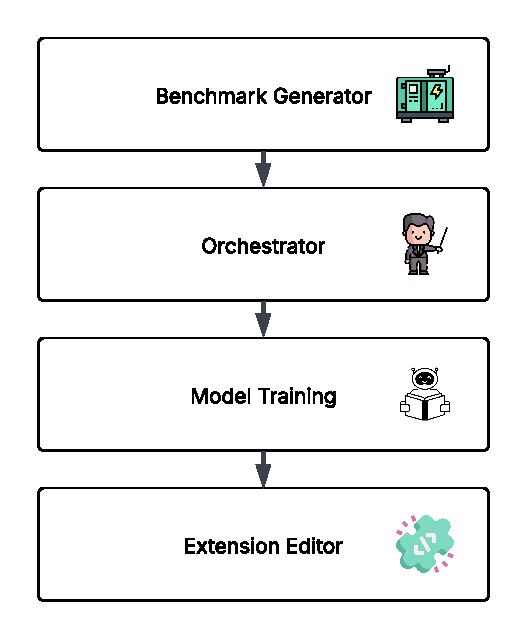
\includegraphics[width = .8 \textwidth]{figures/main_modules.pdf}
  \caption{Main modules}
  \label{fig:main_modules}
\end{figure}
As described in the previous sections, the aim of this work is to make developers aware of the energy consumption of their programs. By using a simple and practical tool, they can quickly and accurately estimate their program's energy consumption. This allows them to get immediate feedback on energy consumption with every code change, facilitating energy-efficient development. It is important to note that this tool serves as a guide, providing energy consumption estimates to raise awareness rather than dictate action. Ultimately, it is up to developers to decide whether to prioritize performance, energy efficiency or any other factor. For example, if a program only needs to run within a certain timeframe and can afford a slight reduction in performance, developers may choose to trade some performance for improved energy efficiency, making more informed decisions thanks to the insights provided by the tool.

To provide this insight to developers it is necessary to build a tool that can provide all of that. The tool needs to be practical, which means that integrating it in an IDE is recommended. With this the developer only needs to download an extension for an IDE and will access to the insights provided by the tool.


The tool will be a VSCode extension built using the Language Server Protocol (LSP). While VSCode may not be the most commonly used IDE for Java projects compared to Eclipse or IntelliJ IDEA, it provides a much simpler and more accessible environment for developing and testing extensions. This will make it accessible to most developers wanting feedback on the energy consumption. To make it fast, it will use static analysis to parse the code into an AST, from there it is capable of analyzing the code and using an inference function it will output the estimated cost.
Although the tool is initially built for VSCode, its use of the LSP standard means it can be extended to other IDEs like Eclipse or IntelliJ IDEA. Since LSP handles the communication between the language server and the development environment, porting the tool to new IDEs would primarily involve adapting the user interface and integration specifics, rather than reworking the core logic.


Many devices rely on Java and the JVM, so it is important that the code they run is energy efficient. Several factors can affect the power consumption of Java applications, including the behavior of the garbage collector and the efficiency of the memory management system ~\cite{10.5555/1267847.1267870} making it difficult to predict the power consumption of Java programs. This unpredictability highlights the need for a specialized tool to accurately measure and analyze power consumption so that developers can optimize their applications for energy efficiency.
Java is an excellent choice for developing this tool because of its high interoperability with various operating systems and its widespread usage across the globe, making it a reliable and option. It has a wide range of useful libraries (JRAPL, JoularJx, Jalen) that help to measure energy accurately, and Java's typing and object-oriented features make the code easier to maintain and extend, so the tool can evolve with new energy metering standards and technologies. 

There are several Java parsing tools available, such as WALA~\cite{wala_main}, SootUp~\cite{sootup_main}, Spoon~\cite{spoon_main} and JavaParser~\cite{javaParser}. WALA and SootUp are primarily designed for analyzing Java Bytecode and are generally more complex to use. For this project, Spoon was chosen because it is a user-friendly tool that facilitates easy retrieval and manipulation of the AST from Java source code. Both JavaParser and Spoon support AST manipulation and code generation. However, Spoon provides a deeper, type-aware metamodel and built-in templating features. These features make Spoon more suitable for generating code that conforms to Java’s syntactic and semantic rules, especially in complex transformation scenarios.

In order to build the extension, it was necessary to build a system architecture capable of providing as final output the functioning tool. The architecture follows different stages, that were deeply analyzed before moving to the next one.
The architecture is divided in 4 main modules, the Program Generator, Orchestrator, Parser and Tool.



\section{Stage 1: Program Generator} \label{sec:work_stage1_program_generator}




To use machine learning models to predict energy consumption, it is necessary to have a large amount of data. This data can be obtained by generating programs that are then executed to collect energy profiles. The program generator is responsible for creating these programs, which are then used to train the machine learning models. The generator is designed to be flexible and adaptable, allowing it to generate a wide variety of programs based on different templates and input parameters. The architecture of the Program Generator can be seen in Figure~\ref{fig:program_generator}.


The program generator works alongside with Java Spoon to make it the more general as possible allowing custom programs to be mass generated.

The generator is capable of generating programs for custom, developer-created, Java classes, as well as for the most common APIs, such as collections interface implementations (Lists, Sets, Maps), and utility classes like Math, Base64, Duration. It can also be configured to analyze all public methods of a class or just specific ones.

\begin{figure}[htbp]%[H]
    \centering
    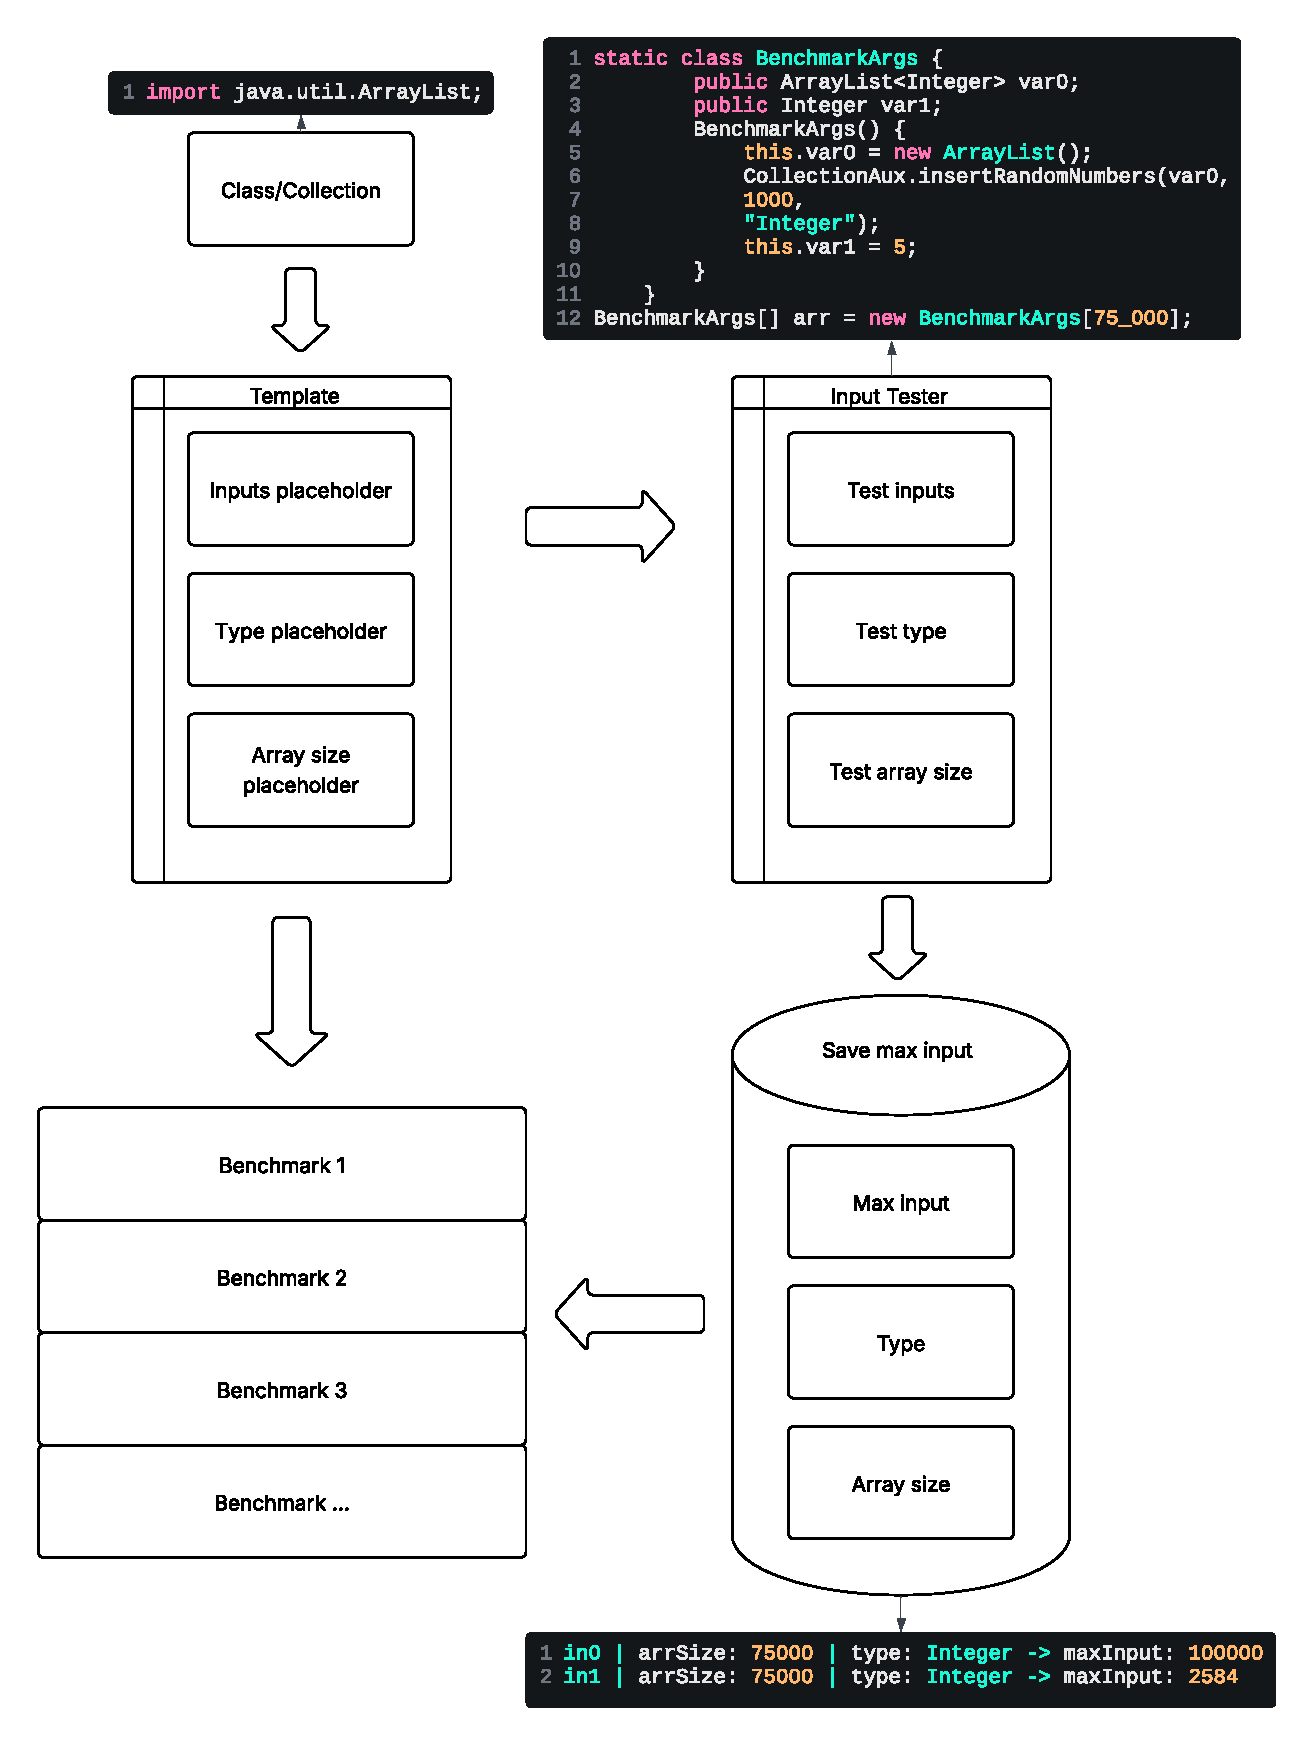
\includegraphics[width = 1 \textwidth]{figures/program_generator.pdf}
    \caption{Program Generator}
    \label{fig:program_generator}
\end{figure}


\subsection{Template Creation} \label{sec:work_stage1_template_creation}

%\FloatBarrier

%\begin{listing}[htbp]
%\begin{minted}[linenos, fontsize=\small, frame=none, bgcolor=white,breaklines=true,breakanywhere=true]{java}
%
%public class ArrayList_add_java_lang_Object_ {
%    public static void main(String[] args) throws Exception {
%        int iter = 0;
%        try {
%            BenchmarkArgs[] arr = new BenchmarkArgs["numberOfFunCalls"];
%            populateArray(arr);
%            TemplatesAux.sendStartSignalToOrchestrator(args[0]);
%            TemplatesAux.launchTimerThread(1100);
%            iter = computation(arr, arr.length);
%        } catch (OutOfMemoryError e) {
%            TemplatesAux.writeErrorInFile("ArrayList_add_java_lang_Object_", "Out of memory error caught by the program:\n" + e.getMessage());
%        } catch (Exception e) {
%            TemplatesAux.writeErrorInFile("ArrayList_add_java_lang_Object_", "Error caught by the program:\n" + e.getMessage());
%        } finally {
%            TemplatesAux.sendStopSignalToOrchestrator(args[0], iter);
%        }
%    }
%
%    static class BenchmarkArgs {
%        public ArrayList<changetypehere> var0;
%
%        public changetypehere var1;
%
%        BenchmarkArgs() {
%            this.var0 = new ArrayList();
%            CollectionAux.insertRandomNumbers(var0, "ChangeValueHere1_changetypehere", "changetypehere");
%            this.var1 = "ChangeValueHere2_changetypehere";
%        }
%    }
%
%    private static void arrayList_add_java_lang_Object_(ArrayList var, changetypehere arg0) {
%        var.add(arg0);
%    }
%
%    private static int computation(BenchmarkArgs[] args, int iter) {
%        int i = 0;
%        while (!TemplatesAux.stop && i < iter) {
%              arrayList_add_java_lang_Object_(args[i].var0, args[i].var1);
%               i++;
%        }
%        return iter;
%    }
%
%    private static void populateArray(BenchmarkArgs[] arr) {
%        for (int i = 0;i < "numberOfFunCalls";i++) {
%          arr[i] = new BenchmarkArgs();
%        };
%    }
%
%    private String input1 = "ChangeValueHere1";
%    private String input2 = "ChangeValueHere2";
%}
%
%
%\end{minted}
%\caption{Example of template for List.add(Object)}            
%\label{lst:template_example}
%\end{listing}

The first step to generate multiple programs is to first create an intermediate template capable of holding the necessary code that will later be used for energy profiling.

To generate programs for a specific class, the user has to input the name of the collection or the name of the custom program it wants to generate. For the collections of Lists, Sets and Maps, the generator is prepared to create more than one implementation of those collections, for example, if the objective is to generate programs to the List collection, the program generator will use the \texttt{ArrayList}, \texttt{LinkedList}, \texttt{Vector} and \texttt{CopyOnWriteArrayList}. The user can also input the name of the method to be analyzed, or simply gather all the available methods in the class, which are then found using Spoon.
After the search for the methods, the generator has access to all the methods it will analyze and their input parameters. Since it has access to the whole class, it can see how its constructors are called, and use them if any of the methods parameters requires. It recursively calls constructors if needed, making it very versatile to use. After identifying the methods that will be targeted, it starts by creating templates for each of them. The templates are Java classes that contain the necessary code to run the method, and placeholders for the inputs and types. The templates are structured so that they can be easily modified later, allowing the generator to create multiple programs based on the same template. The templates are designed following the structure below:

\begin{itemize}

\item Input placeholders: Placeholders that will be later changed with real values for inputs, in this case inputs are variable values. 

\item Type placeholder: Placeholders that will later be replaced with Java wrapper classes.
  
\item Array Size placeholder: Placeholder that will later be replaced with the value of an array size. (more details in~\ref{sec:work_stage2_orchestrator}). 

\end{itemize}

Also, the template is structured so that the programs will work in harmony with the \textbf{Orchestrator}, that will extract the energy profile for each program (see Section~\ref{sec:work_stage2_orchestrator}), so when the placeholders are replaced with actual values, the orchestrator can run the program, and communicate with them.


\begin{listing}[htbp]
\noindent\rule{\linewidth}{0.4pt}
\begin{minted}[linenos, fontsize=\small, frame=none, bgcolor=white,breaklines=true,breakanywhere=true]{java}
static class BenchmarkArgs {
        public ArrayList<changetypehere> var0;

        public changetypehere var1;

        BenchmarkArgs() {
            this.var0 = new ArrayList();
            CollectionAux.insertRandomNumbers(var0, "ChangeValueHere1_changetypehere", "changetypehere");
            this.var1 = "ChangeValueHere2_changetypehere";
        }
    }
\end{minted}
\noindent\rule{\linewidth}{0.4pt}
\caption{Example of variable placeholders creations}            
\label{lst:var_placeholders}
\end{listing}

Templates will have the definitions of a class that holds the necessary variables that the method under evaluation needs to run. Listing~\ref{lst:var_placeholders} shows an example of template to evaluate the method \texttt{List.add(Object)}. It follows the algorithm described in Algorithm~\ref{alg:template_creation_algorithm}. First it creates the list with the smallest constructor possible, then if the variable is a collection (List, Set, Map), or an array, it calls a custom-made method that populates collections with random values of a given type, and then it starts creating variables of parameters that the method \texttt{List.add(Object)} uses. The placeholder \texttt{ChangeValueHere1} will change to a random number, it contains a number \texttt{1} because it represents the input number of the method that will later help the model training understand how inputs can affect energy consumption. The placeholder \texttt{changetypehere} later changes to a type. The template after the transformation can be seen in the Listing~\ref{lst:var_placeholders_replaced}



\begin{algorithm}[htbp]
\caption{Template Creation Algorithm}
\label{alg:template_creation_algorithm}
\begin{algorithmic}[1]
    \Statex \textbf{Given:}
    \Statex \hspace{\algorithmicindent} $collection \coloneqq \{\text{List}\}$, collection selected.
    \Statex \hspace{\algorithmicindent} $ds \coloneqq \{\text{List, Map, Set, arrays}\}$, existent data structures.
    \Statex \hspace{\algorithmicindent} $methods \coloneqq \{\text{add, size, get}, \dots\}$, the set of methods of the classes.

    \Procedure{CreateTemplate}{}
        \State \textit{methods} $\gets$ \Call{getMethods}{\texttt{collection}}
        \ForAll{method \textbf{in} methods}
            \State vars $\gets$ empty list
            \ForAll{parameter \textbf{in} \texttt{method.parameters}}
                \State \textit{var} $\gets$ \Call{ParameterCreation}{\texttt{parameter.type}}
                \If{$parameter.type \in ds$}
                    \State \Call{FillWithRandomValues}{var, maxSizePlaceHolder, typePlaceHolder}
                \EndIf
                \State Append var to vars
            \EndFor
            \State \Call{CreateBenchmarkArrayMethod}{method, vars}
            \State \Call{CreateBenchmarkMethod}{method, vars}
            \State \Call{CreateOrchestratorStartSetup}{}
            \State \Call{CreateComputationMethod}{method, vars}
            \State \Call{CreateOrchestratorEndSetup}{}
            \State \Call{SaveTemplate}{}
        \EndFor
    \EndProcedure

    \Procedure{ParameterCreation}{\textit{type}}
        \If{\Call{IsPrimitive}{type}}
            \State \Return type
        \Else
            \State dependencies $\gets$ \Call{GetConstructorArguments}{type}
            \State args $\gets$ empty list
            \ForAll{dep \textbf{in} dependencies}
                \State arg $\gets$ \Call{ParameterCreation}{dep}
                \State Append arg to args
            \EndFor
            \State instance $\gets$ \Call{Instantiate}{type, args} \Comment{Create an instance, using the smallest constructor.}
            \State \Return instance
        \EndIf
    \EndProcedure
\end{algorithmic}
\end{algorithm}



\begin{listing}[htbp]
\noindent\rule{\linewidth}{0.4pt}
\begin{minted}[linenos, fontsize=\small, frame=none, bgcolor=white,breaklines=true,breakanywhere=true]{java}
static class BenchmarkArgs {
        public ArrayList<Integer> var0;

        public Integer var1;

        BenchmarkArgs() {
            this.var0 = new ArrayList();
            CollectionAux.insertRandomNumbers(var0, 1000, "Integer");
            this.var1 = 10;
        }
    }
\end{minted}
\noindent\rule{\linewidth}{0.4pt}
\caption{Example of variable placeholders replaced}            
\label{lst:var_placeholders_replaced}
\end{listing}



It is worth mentioning that the types used by the generator are the Java wrapper classes, which are object representations of the primitive types. Using these types it is possible to achieve a more general generator, as every program can use them and if other custom types were used it would make the generator more complex and not general.

What mostly differs from template to template is the number of variables used, because different methods have different parameters, so the template can have more or less input placeholders, also the type placeholder changes according to the methods types and parameters.


Creating the template for each method allows cutting off time of the program generation by only having to replace values of the placeholders instead of needing to create the whole program all over again, since the programs for the same method only differ in inputs, types and array size, maintaining all the structure.

\subsection{Input Tester} \label{sec:work_stage1_input_tester}

An important aspect of the program generator are the inputs it generates. Every method has its on funcionality that may be dependent on the input values.  To be able to better generalize, it is important to find the method input values upper limit. Knowing the maximum size that different parameters can have is fundamental as it needs to be representative, so the energy profiles can cover more cases, but not to large so that the programs start to get out of memory or taking too much time to complete.
The limit definition works by using binary search. It has an inital threshold on the inputs (e.g., 1-100,000 to numerical values) and it starts by trying to run the program with the half of the maximum upper limit threshold (e.g., 50,000). 

It can be important, for pratical reasons, to impose a threashold on the execution time (in this project, we established the threshold as 10 seconds based on empirical experimentation). If the program runs successfully, it will increase the input by half, and if it fails, it will decrease the input by half. This process continues until the maximum value for the input is found.

If the method that is being tested has more than one input, the input tester is responsible to find the upper limit for each parameter individually. First it sets all the input values to 1 and then starts the binary search individually for each of the parameters one by one while leaving the other parameters with the value of 1. Although this is a simplification, this method avoids having to find multiple combinations of parameters which would increase the time complexity exponentially. More robust solutions (such as using a combinatory search) could be implemented in the future. Nevertheless, even using the simplified solution, the process of finding the max inputs is time-consuming. To improve its performance, when the maximum value is found, the values of the input type, maximum value and order (e.g., first, second or third parameter), are stored in a file. This makes subsequent executions much faster. It is worthy to mention that the maximum inputs found depend heavily on the machine where the program generation is taking place, as different hardware will change the maximum values allowed for the inputs. Example 1 illustrates how the input tester works for the method \texttt{List.add(index, Element)}.

\begin{tcolorbox}[
    title=Example 1: Input Testing Process for \texttt{List.add(index, Element)},
    colback=gray!5!white,
    colframe=gray!75!black,
    fonttitle=\bfseries,
    breakable,
    label={box:add-method-testing}
]

Consider analyzing the \texttt{add} method of a list with the following parameters:
\begin{itemize}
    \item \texttt{arg0}: Size of the list (integer)
    \item \texttt{arg1}: Index at which to insert the new value (integer)
    \item \texttt{arg2}: Value to be added (integer)
\end{itemize}

\textbf{Step 1 – Varying \texttt{arg0} (list size):}

\begin{itemize}
    \item Iteration 1: \texttt{arg0 = 25,000}, \texttt{arg1 = 1}, \texttt{arg2 = 1}
    \item Iteration 2: \texttt{arg0 = 12,500}, \texttt{arg1 = 1}, \texttt{arg2 = 1}
    \item Iteration 3: \texttt{arg0 = 6,250}, \texttt{arg1 = 1}, \texttt{arg2 = 1}
    \item $\vdots$
    \item Final Iteration: \texttt{arg0 = 1,700}, \texttt{arg1 = 1}, \texttt{arg2 = 1}
\end{itemize}

\textbf{Step 2 – Varying \texttt{arg1} (index):}

\begin{itemize}
    \item Iteration 1: \texttt{arg0 = 1}, \texttt{arg1 = 25,000}, \texttt{arg2 = 1}
    \item Iteration 2: \texttt{arg0 = 1}, \texttt{arg1 = 12,500}, \texttt{arg2 = 1}
    \item $\vdots$
    \item Final Iteration: \texttt{arg0 = 1}, \texttt{arg1 = 1}, \texttt{arg2 = 1}
\end{itemize}

{Note: Since the list size (\texttt{arg0}) remains 1, the maximum valid index (\texttt{arg1}) is constrained to 1. This reveals a limitation in the input testing approach.}

\textbf{Step 3 – Varying \texttt{arg2} (value to be added):}

\begin{itemize}
    \item Iteration 1: \texttt{arg0 = 1}, \texttt{arg1 = 1}, \texttt{arg2 = 25,000}
    \item Iteration 2: \texttt{arg0 = 1}, \texttt{arg1 = 1}, \texttt{arg2 = 37,500}
    \item $\vdots$
    \item Final Iteration: \texttt{arg0 = 1}, \texttt{arg1 = 1}, \texttt{arg2 = 100,000}
\end{itemize}

\textbf{Final stored input limits:}
\begin{itemize}
    \item \texttt{arg0} — \texttt{integer} — \texttt{1,700}
    \item \texttt{arg1} — \texttt{integer} — \texttt{1}
    \item \texttt{arg2} — \texttt{integer} — \texttt{100,000}
\end{itemize}

\end{tcolorbox}


The fact that the input has a pre-determined range it allows using binary search which makes the search much faster than linear search.
Nevertheless, the input search does not come without some limitations. First it is constrained to identifying valid input values within the range. As an example, throughout this project we dealt frequently with lists and collections, which require a minimum size of 1 to function correctly. Although this value can be changed in the future, for now it ensures compatibility with most common data structures. The higher bound was chosen due to empirical evidences, as larger input values would lead to limitating execution times and memory crashes. Another constraint is on how the input handles multiple parameter methods. During its search for a valid input, it needs to fix all the other parameters that is not searching, with a default value (typically the lower bound). This approach simplifies the testing process and improves efficiency by avoiding the exponential complexity of testing all possible parameter combinations. However, it will introduce limitations in cases where the parameters are interdependent, which can lead to not estimating the real highest input possible. 
Despite these limitations, the input search plays a crucial role in ensuring that the program generator produces viable test cases. By identifying input ranges that are both valid and computationally achievable, it reduces the unusable generated programs (e.g., due to timeouts or crashes), and maximizing the number of generated programs, that can be used for energy profiling.



\subsection{Program Generation} \label{sec:work_stage1_program_generation}

Finally, when the templates are created, and the maximum inputs are found the program generation can finally begin. This part consists on picking every template created and replacing the placeholder values with actual values created by a random number generator. It follows the algorithm described in Algorithm~\ref{alg:template_fullfillment_algorithm}

It starts by looping through the types and changing them to the Java wrapper classes, then it loops through the array size. Lastly, it loops through the input sizes determined by the input tester and can repeat this process a configurable number of times. By increasing the number of iterations, results in more programs being generated with random inputs, constrained by the previously identified input bounds. 




\begin{algorithm}[htbp]
\caption{Template Fullfillment Algorithm}
\label{alg:template_fullfillment_algorithm}
\begin{algorithmic}[1]
    \Statex \textbf{Given:}
    \Statex \hspace{\algorithmicindent} $templates$, list of templates previously generated.
    \Statex \hspace{\algorithmicindent} $types \coloneqq \{\text{Integer, Double, Long, Float, Short, Character }\}$, types to be replaced.
    \Statex \hspace{\algorithmicindent} $arraySize \coloneqq \{\text{75\,000, 100\,000, 150\,000}\}$, array sizes to be used.
    \Statex \hspace{\algorithmicindent} $template.maxInputs $, each template has a maximum input file associated to it.
    \Statex \hspace{\algorithmicindent} $iterations $, number of iterations for the input loop.

\Procedure{FullfillTemplate}{}
    \ForAll{template \textbf{in} templates}
        \ForAll{type \textbf{in} \texttt{types}}
            \State program $\gets$ \Call{Replace}{template, "typePlaceHolder", type}
                \ForAll{arraySize \textbf{in} \texttt{arraySizes}}
                    \State program2 $\gets$ \Call{Replace}{program, "arraySizePlaceHolder", arraySize}
                        \For{$i \gets 0$ \textbf{to} \texttt{iterations}}
                            \State program3 $\gets$ \Call{replaceValues}{program2, template.maxInputs}
                            \State \Call{SaveToFile}{program3}
                        \EndFor
                \EndFor
        \EndFor
    \EndFor
    
\EndProcedure

\vspace{1em} 

\Procedure{ReplaceValues}{program, maxInputs}
    \State valuesToReplace $\gets$ \Call{FindStringsToReplace}{program, placeholderPattern}
    \For{$i \gets 0$ \textbf{to} \Call{Size}{valuesToReplace} - 1}
        \State value $\gets$ valuesToReplace[i]
        \State type $\gets$ \Call{ExtractType}{value}
        \State max $\gets$ maxInputs[i]
        \State min $\gets$ \Call{Min}{1, max}
        \State newValue $\gets$ \Call{GetRandomValue}{type, min, max}
        \State program $\gets$ \Call{Replace}{program, value, newValue}
    \EndFor
    \State \Return program
\EndProcedure

\end{algorithmic}
\end{algorithm}

This process easily generate thousands of programs which are crucial to train machine learn models that are able to predict energy consumption. When generating programs, a number is chosen to balance the requirements for effective model training while minimizing the time spent on input testing and collecting energy profiles. Afterwards, that the programs are ready to be compiled and used.



\section{Stage 2: Orchestrator} \label{sec:work_stage2_orchestrator}




Having all the programs generated, it is possible to move to the next stage. Gathering the energy profiles for each of the generated programs. 
Energy profiles~\cite{10.1145/2884781.2884869,8816747} are an established way to organize energy consumption data. They will be the main data source of the machine learning models to obtain accurate results. To reduce the complexity of this task, a process was implemented, illustrated in Figure~\ref{fig:orchestrators_workflow}. This process automates the task while taking into account what was mentioned in Section~\ref{sec:background_benchmarking}.

As described in the Section~\ref{sec:background_energy} there are several tools capable of performing dynamic energy measurements.

PowerJoular has good features that caught our attention, for example being a command line tool that could be easily integrated in almost every programming language, it stores the energy used in a CSV file, capable of only reading energy of running processes and so on, as explained before in Section~\ref{sec:background_energy}.

Since PowerJoular is a command line tool, it is launched as a process, and then it can be killed whenever needed because it is a process as well. This allows to measure not only programs/processes energies but have a more precise measurement, as it is possible to call PowerJoular to measure a specific computation and then kill it when the computation is finished.

With all of this in mind a process was built. The process uses an orchestrator that is responsible for invoking the target program and the measurement tool (PowerJoular) to accurately measure the energy consumption of the program or the specific computation being analyzed within it.


One challenge in measuring energy consumption is that computation often completes too quickly to capture accurately. It is hard to measure a single operation of, for example, a \texttt{List.\allowbreak add(Object)} with most tools, as it simply to fast for the tool to capture, and if the tool was able to capture it, the energy measured could have too much noise to be considered. Our solution was to loop through the method until the tool is capable of getting its energy and then dividing the total energy by the number of times it looped. 
This solution, although effective, introduces potential errors that need to be addressed.

By approaching the measurements with the loop technique, first we need to create the variables needed for the method target to analysis, like shown in the Listing~\ref{lst:var_placeholders} \wo{dê exemplos}. However, because, the methods are treated like a black box, it is not possible to know what the methods are going to do with the parameters or with its variables. {\color{blue} For example, the method \texttt{List.size()} has no parameteres, and return the size of the list. In this case the functioning of the method is known, and it is noticeable that the attributes of the object will not change, as the method simply reads and returns a value.

However, this raises problems with other methods, such as \texttt{List.add(Object)}. This method will insert values in the list, increasing its size. This increase in size can lead to different behavior of the method as the internal object changes in each iteration. In this case, inserting into a smaller list can produce different measurements of inserting into a larger list.}

Now, suppose we have a method called \texttt{sort} that takes a randomly ordered list and sorts it. This introduces a problem when measuring its energy consumption. On the first run, the method will sort the unsorted list, which may take significant time depending on the randomness of the data and the sorting algorithm used. However, on subsequent runs with the same list, the input is already sorted, meaning the sort method will likely complete much faster or with minimal effort. This difference can result in misleading or inconsistent measurements.

To prevent this side effect from happening we designed a solution that consists of creating an array that holds the parameters, that can be seen in the Figure~\ref{fig:array}. The necessary parameters to execute the method are created and stored into the array. They are exactly copies with different refereces. Now, if one of the elements is changed during its execution on the method, it will not affect the other's execution. Since this approach increases memory usage due to multiple copies, we empirically selected array sizes (75,000, 100,000, and 150,000) to balance between avoiding out-of-memory errors and ensuring the computation runs long enough for PowerJoular to record energy measurements. PowerJoular by default needs to run for 1 second to create the CSV file that has the energy used for the target process, so these sizes aim so that looping the array takes at least a second. In some cases, the CSV file may not be generated because the loop executes too quickly. In such instances, the energy reading will be assumed to be 0 J, as the execution was too fast to record a value.


\begin{figure}[htbp]
  \centering
  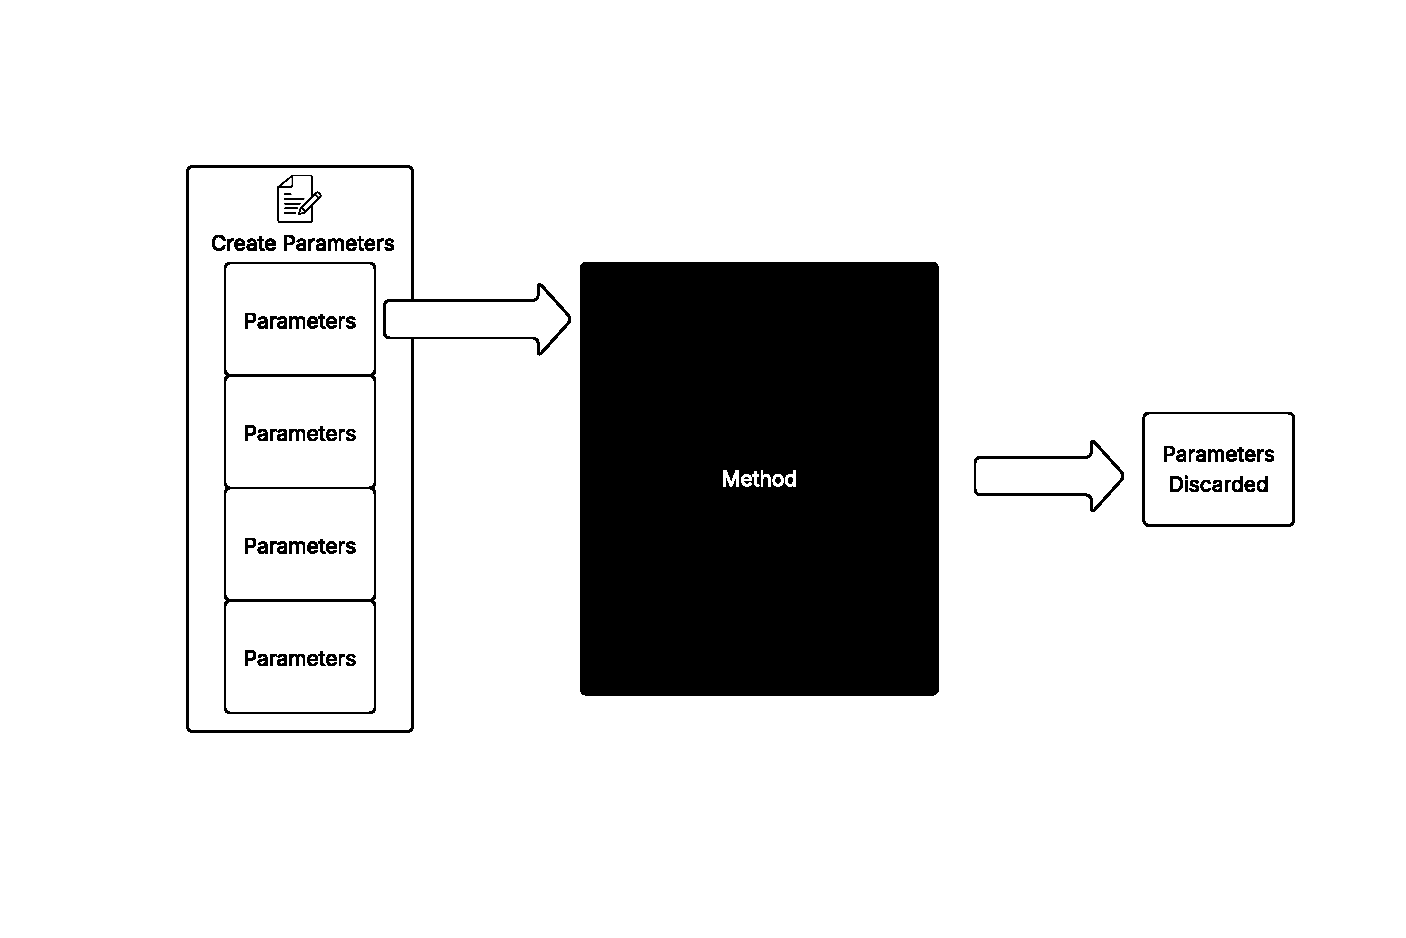
\includegraphics[width = 1 \textwidth]{figures/array.pdf}
  \caption{Array example}
  \label{fig:array}
\end{figure}

To be able to collect some faster executions, the original PowerJoular was modified to allow customizable measurement durations, enabling readings at intervals shorter than the default 1 second, such as 100ms, which provides greater flexibility and finer granularity in energy profiling.

The computation method shown in Listing~\ref{lst:Computation_method} illustrates how each profiling method operates independently of the specific method being evaluated. It attempts to execute the target function repeatedly for approximately one second. In this particular case, the target function performs the operation \texttt{var.add(arg0);} and returns the number of iterations completed, which is then used for further calculations.

\begin{listing}[htbp]%[H]
\noindent\rule{\linewidth}{0.4pt}
\begin{minted}[linenos, fontsize=\small, frame=none, bgcolor=white,breaklines=true,breakanywhere=true]{java}
private static int computation(BenchmarkArgs[] args, int iter) {
        int i = 0;
        while (!TemplatesAux.stop && i < iter) {
              arrayList_add_java_lang_Object_(args[i].var0, args[i].var1);
               i++;
        }
        return iter;
    }
\end{minted}
\noindent\rule{\linewidth}{0.4pt}
\caption{Computation method}            
\label{lst:Computation_method}
\end{listing}


With the process structure now defined, we can proceed to explain how it functions.

The workflow of this step can be described as follows:


\begin{figure}[htbp]
  \centering
  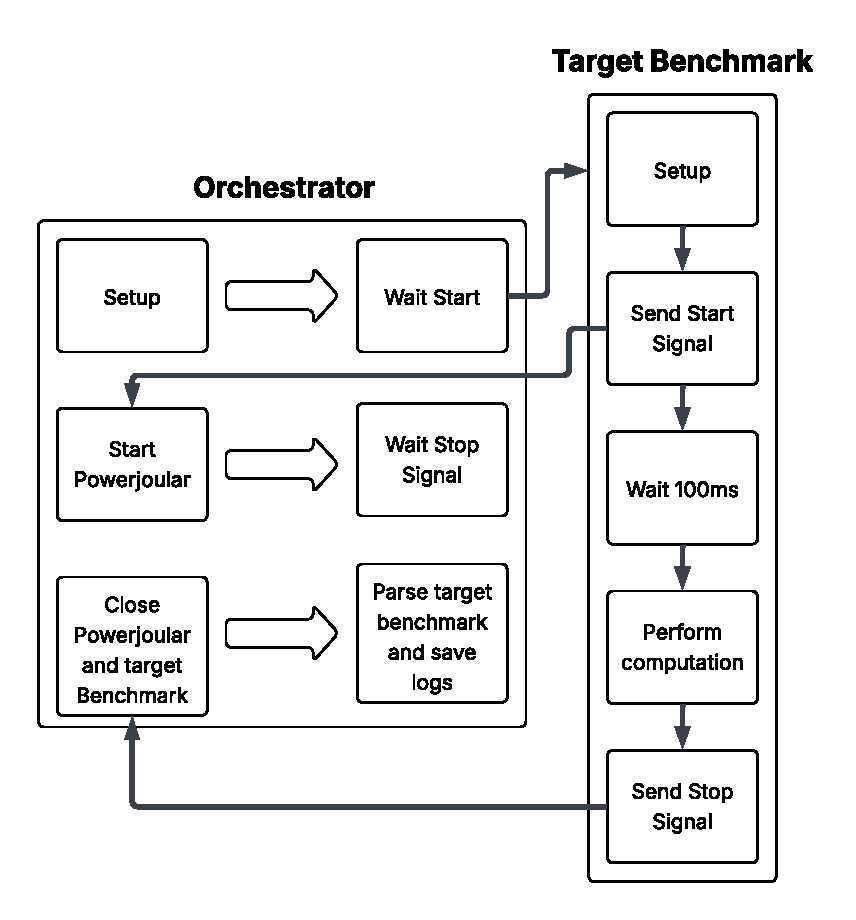
\includegraphics[scale = 0.7]{figures/orchestrators_process.pdf}
  \caption{Orchestrator Workflow}
  \label{fig:orchestrators_workflow}
\end{figure}

\begin{itemize}
  \item The orchestrator launches a command to start the target Java Program and waits a signal.
  \item The Java program starts and setup the necessary elements to run (creating all the variables, reading/writing files, populating the array, etc.) and then before starting the computation it wants to measure, it sends a start signal to the orchestrator to start monitoring, and waits for 100 milliseconds.
  \item The orchestrator receives the start signal and reads the PID, which is stored in a file during the target program setup. Finally, it starts PowerJoular using that PID. Then it waits for the stop signal.
  \item The Java program will run until it finishes the computation. The computation runs for a maximum of one second. Then the number of iterations are stored in a file and the stop signal is sent back to the orchestrator.
  \item The orchestrator on receiving the stop signal, first stops PowerJoular and then stops the target program, if needed. Then it parses the target program to extract its features, combines them with the energy information stored in the files created by PowerJoular, stores it in a CSV file.
\end{itemize}

All these steps are performed for each generated program. At the end of the process, a log file is created containing key information, including all the programs used, the PowerJoular files generated, temporary files, error logs, and features.


\section{Stage 3: Model Training} \label{sec:work_stage3_model_training}

Now, that all the energy profiles are collected it is possible to finally start training the models. As explained in \ref{sec:background_machine_learning} there are a lot of possible ways of using machine learning, however in this case the approach that best fit our need is supervised machine learning. So, some models were trained to see how good they performed using the data collected.

First there is a merge of features. While each method is initially trained individually, it is not useful to treat LinkedList.add(Object) and ArrayList.add(Object) as entirely separate cases. Both represent the same List.add(Object) method, differing only in their characteristics specific to their implementation. Therefore, once all energy profiles have been collected, a merging step is performed to consolidate these related methods.

All these features are stored in a new CSV and for the python program in a Data frame, to be processed.

This part was developed in python using some libraries specialized on machine learning, like scikit-learn (sklearn)~\cite{scikit-learn} which contains some models and functions to evaluate the models, and PySR~\cite{cranmer2023interpretablemachinelearningscience} which was already explained in \ref{sec:background_machine_learning} an is also already implemented.

In this phase the models tested were: Decision Tree Regressor, Random Forest, Gradient Boosting, Linear Regression, and PySR.

First the values of the MSE and R2 are evaluated by the default values of sklearn, then in a second pass, GridSearch was used, which is a function of sklearn that tries to find the best parameters for a model. After that the scores and models are saved. The GridSearch does not work with PySR as they are from different libraries so, the parameters for PySR were manually set.

In the end the chosen model was PySR as it can represent the predictions in expressions which can help the users to try to understand why the code is using more energy. It has a nice feature of allowing to balance complexity and accuracy. And can easily be used in another code language as it is represented as a mathematical expression.





%\section{Step 3: Implementation and testing} \label{sec:work_step3_implementation_and_testing}
%
%Once the main components of the tool are built, they need to be assembled into the extension. When using it, the developers should be able to see the total energy estimate of their code in the IDE, and it should also show the estimates for each function and its most energy consuming lines.
%The estimate alone may be enough to understand if the code is high or low in energy consumption, for example, if the developer has two implementations of the same function and they both give different values, it may be easy to understand which one consumes the most. However, this may not always be the case, so the tool will also provide some information to help the developer know how good or bad the energy efficiency of the code is.
%
%Another important step is to test and ensure that the tool performs as expected on most machines, delivers the most accurate estimations possible, and undergoes a final comparison with other tools to evaluate its effectiveness.
%

% trabalho realizado (podem ser vários capítulos)
\chapter{Results}\label{chapter:results}\textcolor{blue}{Tudo novo}

%\section{The issue with inconsistent energy readings} \label{sec:results_the_issue_with_inconsistent_energy_readings}

At the beginning of the experiment, some tools were tested to observe their behavior, understand how to use them, and determine which one best suited the needs of the project.

During the initial testing, a Python framework designed to facilitate experiment measurements was used~\cite{S2_Group_Experiment_Runner}. The framework included an initial test template that used PowerJoular to measure energy of programs. While using the template and testing the framework some bugs and unexpected results were found, some of which were due to misuse of the framework.
Due to these issues, a simpler orchestrator was developed. Although it performed the same core function as the original framework, measuring energy consumption, it was more straightforward, focusing exclusively on energy measurement rather than providing a general-purpose solution. This new orchestrator was implemented in Java.

However, some discrepancies were observed between the energy values measured by the Java and Python frameworks. This was unexpected, as both used the same energy measurement tool (PowerJoular) and measured the same program in the same way. Still, the Python framework consistently reported lower energy values than the Java version.
To investigate which tool was causing the inconsistency, two more orchestrators were implemented. A simplified custom version of the Python framework was also created. In total, four orchestrators were developed: Java, Python, C, and Bash. All four performed the same process, calling PowerJoular to measure the energy usage of a Java program.
This setup represents an early iteration of the approach later detailed in Section~\ref{sec:work_stage2_orchestrator}, which utilized signal-based control to ensure that the measurement tool only ran during the exact computation period being measured.

\begin{figure}[htbp]
  \centering
  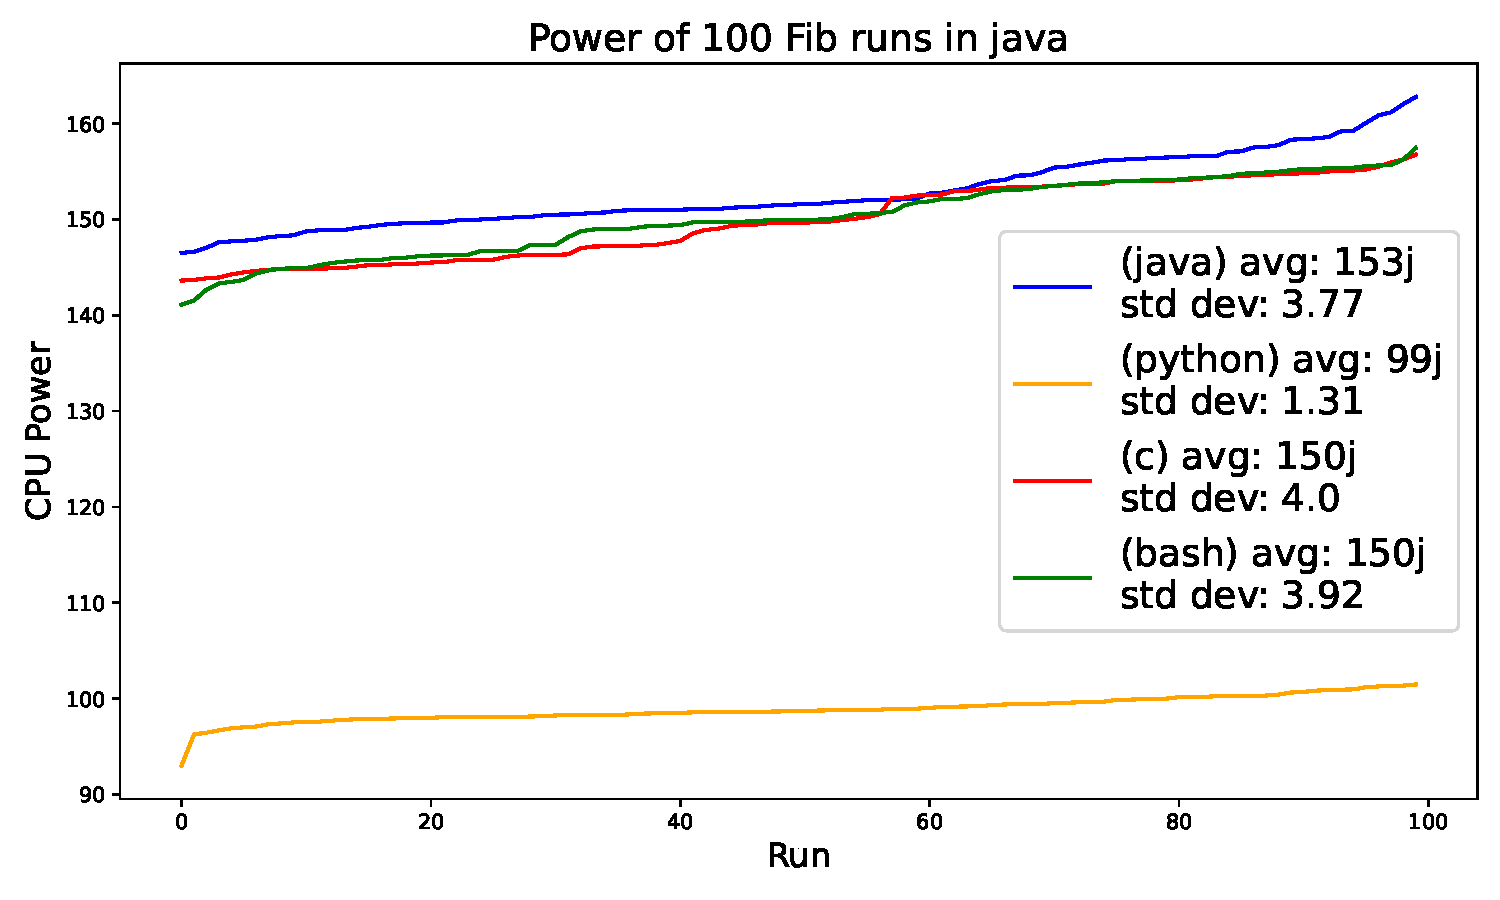
\includegraphics[width = .8 \textwidth]{figures/4_orchs_comparison.pdf}
  \caption{Orchestrators Comparison}
  \label{fig:4_orchs_comparison}
\end{figure}

To better understand the inconsistencies, Figure~\ref{fig:4_orchs_comparison} details the differences.
The figure contains 100 runs of the Fibonacci recursive program written in Java and order by the less energy to the highest energy. And it shows the energy reads for the four different orchestrators used. The labels contain the average energy values and its standard deviation.

It is noticeable that the Python orchestrator read energy values lower than the other orchestrators. Further analysis of the orchestrators revealed a notable difference in behavior. When the Python orchestrator was running, both the parent and child processes consumed CPU resources. In contrast, the other orchestrators (Java, C, and Bash) showed CPU usage only in the child process. This disparity may explain why PowerJoular reported lower energy consumption for the Python orchestrator. Since the CPU load was shared between the parent and child processes, PowerJoular, which measures energy only for the child process (the target Fibonacci program), captured less total energy usage.
Since the experiment runner included an example demonstrating how to use the framework with PowerJoular, the authors were made aware of this potential conflict when launching PowerJoular from Python.


\section{Models Metrics} \label{sec:models_metrics}

For the final version of the tool, models were trained on methods from the Java collections framework, specifically focusing on the \texttt{List} and \texttt{Map} interfaces. Data for these methods was generated, collected, and used to train the models. With the models in place, it is now possible to evaluate their performance using metrics such as R² and Mean Squared Error (MSE), based on the features extracted during data collection.

\begin{figure}[htbp]
  \centering
  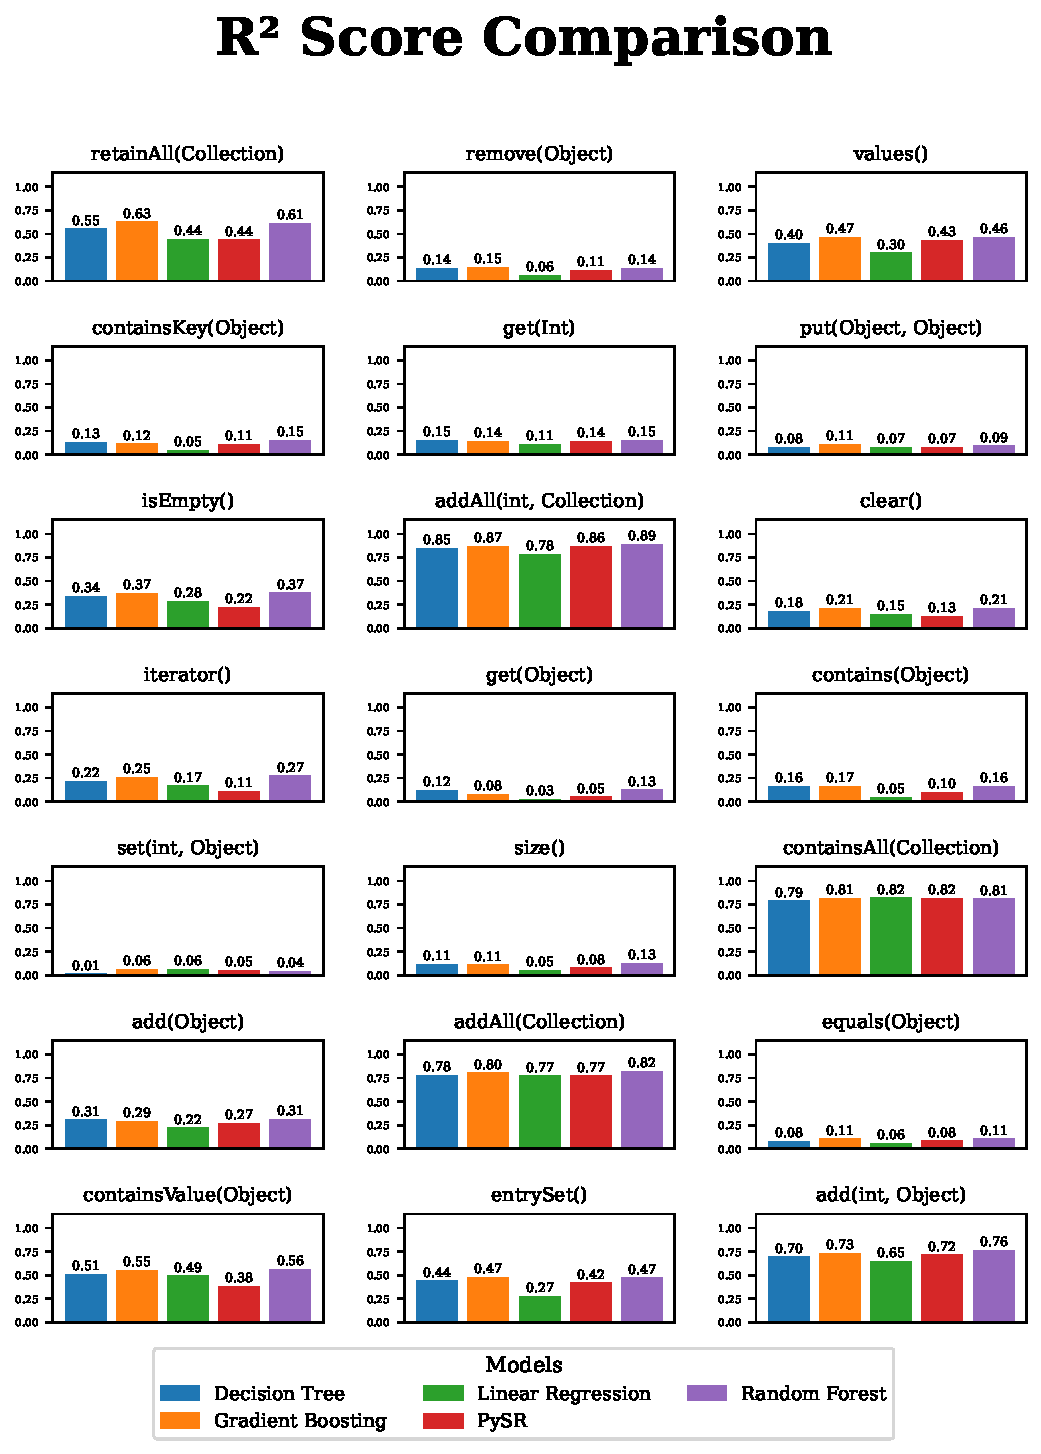
\includegraphics[width=0.85\textwidth]{figures/r2_comparison.pdf}
  \caption{R² Comparison (Higher is better)}
  \label{fig:r2_comparison}
\end{figure}




\begin{figure}[htbp]
  \centering
  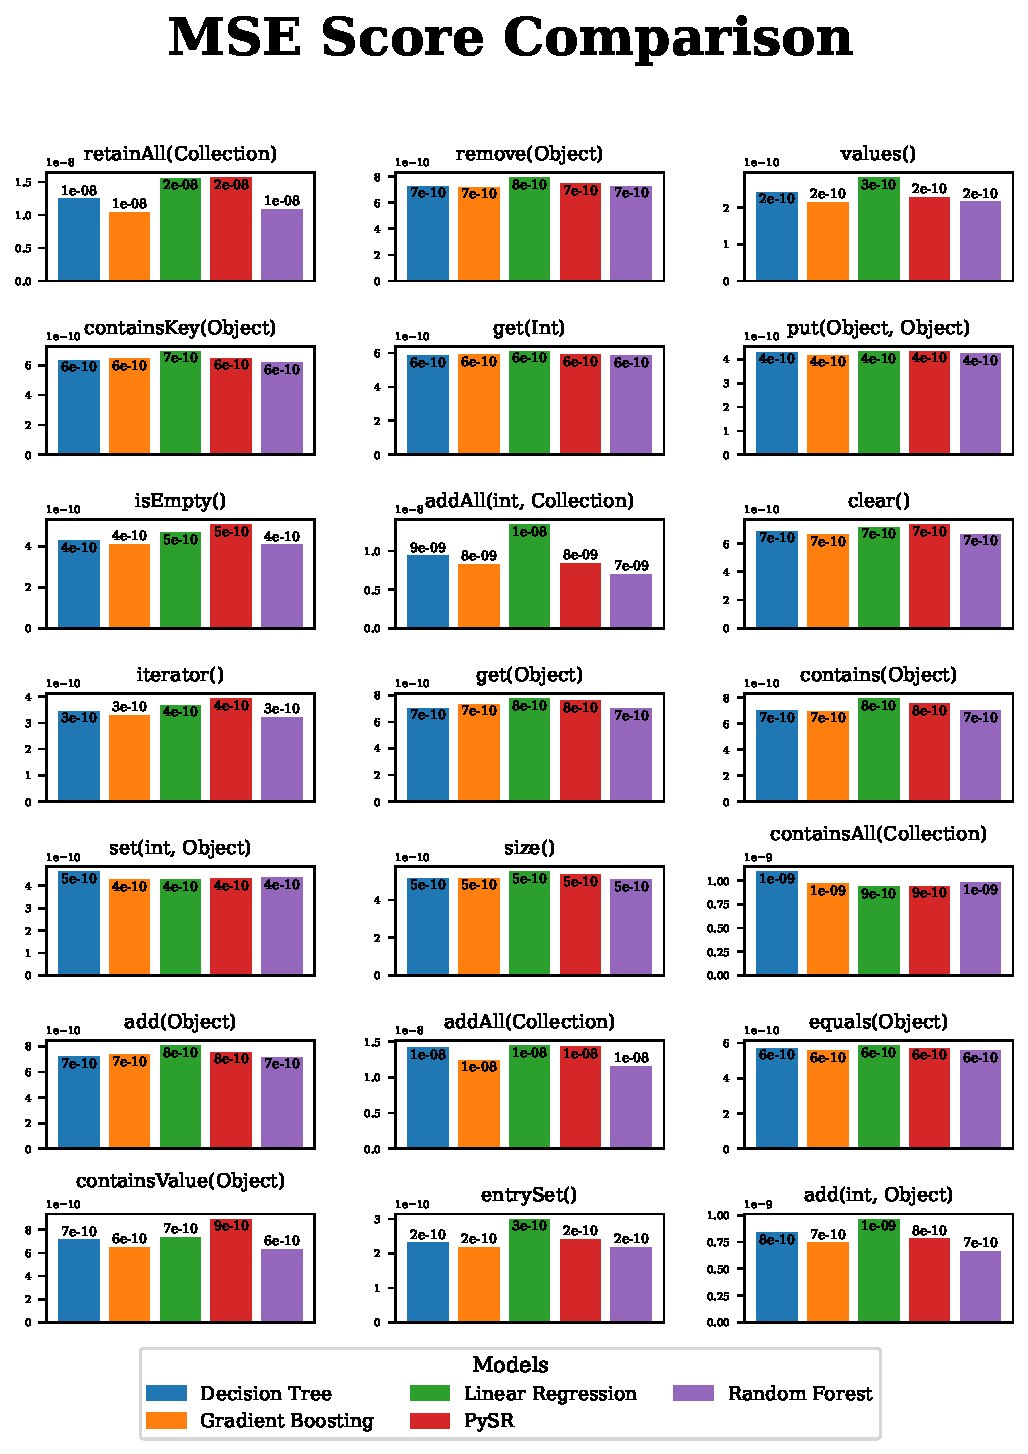
\includegraphics[width=0.85\textwidth]{figures/mse_comparison.pdf}
  \caption{MSE Comparison (Lower is better)}
  \label{fig:mse_comparison}
\end{figure}

The results of the R² can be seen in the Figure~\ref{fig:r2_comparison}.
Ideally the best score is 1, meaning that the model can get 100\% of the prediction right, however that is not possible in most cases, and this project is not an exception to the rule. It is noticeable that most values are really low (bellow 0.8), which means that the model cannot predict the energy very well for some methods. The best models were for the method \texttt{addAll()} and \texttt{containsAll()} of the List collection, which got an R² of around .8 for most models, meaning that for those 3 methods on average the predictions will be 80\% correct.

For the other methods the scores were lower. The explanation found for this result was the following:


\begin{figure}[htbp]
  \centering
  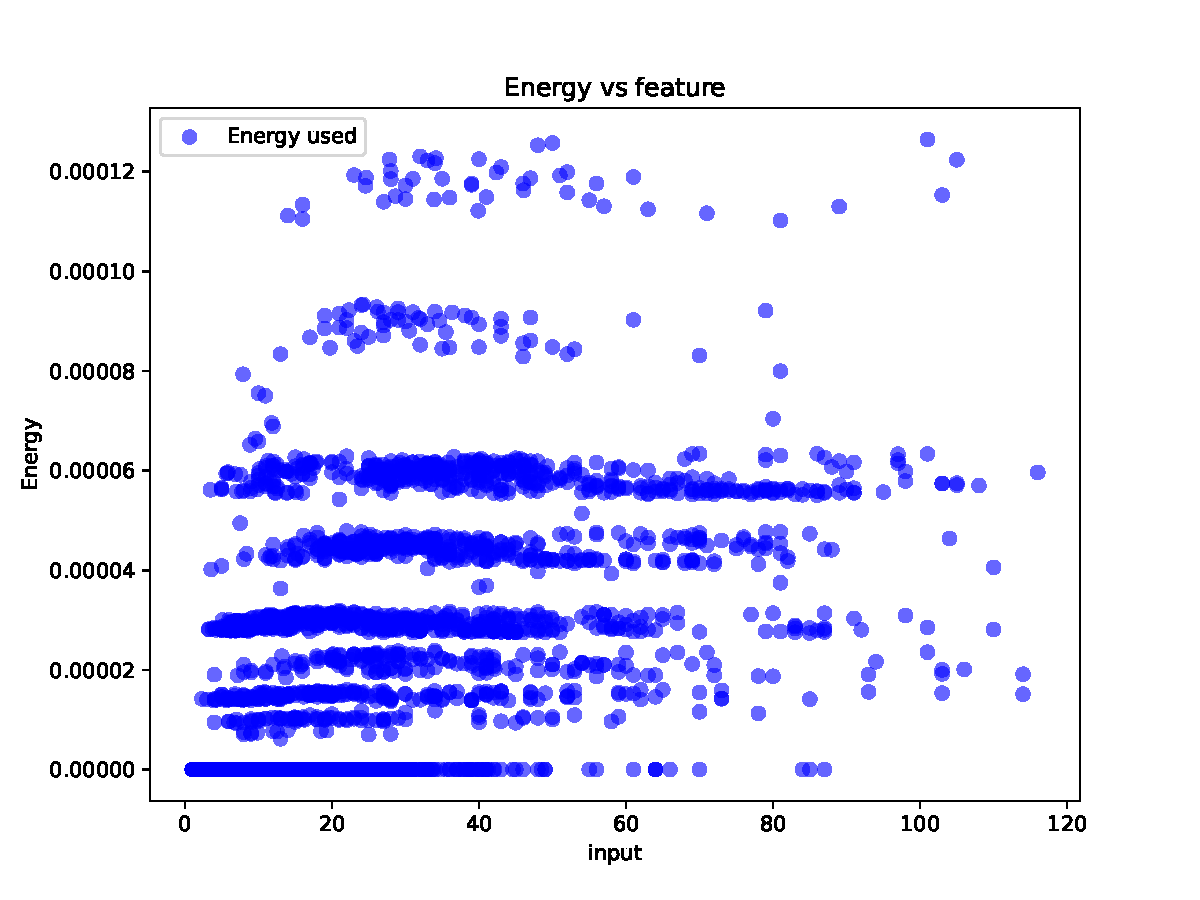
\includegraphics[width = .8 \textwidth]{figures/size_energy.pdf}
  \caption{Energy for the \texttt{List.size()} method with different list sizes.}
  \label{fig:size_energy}
\end{figure}

The 3 methods with the most accuracy were the ones that generated bigger energy outputs, because the methods were computationally more powerful than the others. This made it so that bigger inputs would result in bigger energy outputs, and make the models more easily find a pattern to predict the energy. As for the other models, since a bigger input would not mean a bigger energy output, the model, might had some difficulties predicting the energy. This does not mean that a lower R² will completely make the model unusable for some methods, as their MSE, that can be seen in the Figure~\ref{fig:mse_comparison} is not high, meaning that even when failing to predict the energy of the method, the failed prediction will not be far away as one might expect. For example, if a model has an MSE of $1 \times 10^{-10}$ and predicts the energy usage to be $1~\mathrm{J}$, then even if the prediction is not exact, the true value is likely within $\pm \sqrt{1 \times 10^{-10}} = \pm 1 \times 10^{-5}~\mathrm{J}$ of the prediction, indicating accurate performance despite a potentially low R². 

Another factor that may contribute to low R² scores is the behavior of the energy measurement tool when applied to certain methods. For instance, some methods, such as \texttt{size()}, do not require more computational effort as the collection size increases. Whether the collection has one element or one million, the method executes in roughly the same amount of time. Consequently, the energy consumption remains nearly constant, regardless of the input size. Since these methods complete very quickly and consume very little energy, even minimal measurement noise can significantly affect the recorded values. Figure~\ref{fig:size_energy} illustrates this effect: although an increase in energy with input size is typically expected, the recorded energy values for \texttt{List.size()} remain considerably flat. While this example isolates a single feature, and other features also influence energy consumption, input size is often the most significant. This observation suggests that for low-energy, low-variance methods, measurement noise can impact the signal, making accurate energy prediction particularly challenging.


Nonetheless, the lower R² scores should be addressed, and what can be done to improve the results of these models is to have the program generator create higher inputs, so the energy profiles also have outputs with higher energy, making the energy predictions more accurate. Then, since most of the predictions depend on the input, it means the other features do not have such higher impact, so it is also important to pick better features and remove others that might not be interesting. 



In general, most of the models present similar scores, however the chosen one was PySR. As it can represent the predictions in expressions which can help the users to try to understand why the code is using more energy. It has a nice feature of allowing to balance complexity and accuracy. And can easily be used in another code language as it is represented as a mathematical expression.
The fact that most models present similar results, ranging from advanced models like Random Forest and Gradient Boosting to simple models like Linear Regression, suggests that features used in the model likely do not capture highly nonlinear or complex relations. This indicates that energy consumption behavior in analyzed approaches can be reliably captured by simple relations. As a result, the set of features cannot offer the richness or variability needed for distinguishing more subtle energy behavior. This does not mean that the learning problem is simple, rather, it indicates that the available features may fail to express potential nonlinear patterns of energy consumption. To improve prediction performance and enable more effective use of expressive models, future work should incorporate features capable of highlight the complexity of predicting energy usage.



\section{Predicted vs. Measured Energy} \label{sec:predicted_vs_measured_energy}

Since the extension has been built, we can present the results and evaluate how accurately the tool estimates energy consumption compared to real measurements obtained using PowerJoular. Since the energy profiles were generated on a specific hardware setup (see Table~\ref{tab:hardware_specs}), the resulting models are adjusted to that particular system. If the tool were run on a different machine, the absolute energy values would likely differ due to variations in hardware characteristics. However, the relative differences in energy consumption between operations are expected to remain consistent. For instance, if \texttt{TreeMap} consumes more energy than \texttt{HashMap} on one system, the same trend will likely hold on another system, even if the exact energy values vary.

\begin{listing}[H]
\noindent\rule{\linewidth}{0.4pt}
\begin{minted}[linenos, fontsize=\small, frame=none, bgcolor=white,breaklines=true,breakanywhere=true]{Java}
    ArrayList<Integer> l = new ArrayList<>();
    ArrayList<Integer> l2 = new ArrayList<>();
    l.addAll(l2);
\end{minted}
\noindent\rule{\linewidth}{0.4pt}
\caption{Code example}            
\label{lst:code_example}
\end{listing}

To test if the extension tool is accurate, the energy measurement needs to be run in the same machine were the data was collected.
For this a simple program was developed, Listing~\ref{lst:code_example}, more like simple Java instructions, of just creating two lists (both with size 1000) and using the method \texttt{addAll(Object)} and checking if the prediction matches the actual measurement.

\begin{table}[htbp]
  \centering
  \label{tab:energy_comparison}
  \footnotesize
  \begin{tabular}{>{\raggedright\arraybackslash}p{4cm}ccc}
    \toprule
    Method & Actual Energy Range (J) & Predicted Energy (J) & Prediction Error (\%) \\
    \midrule
    \texttt{addAll(Object)} & 4.9e-4 -- 5.1e-4 & 5.51e-4 & 10.2 \\
    \midrule
    \texttt{addAll(Object)} + \texttt{size()} + \texttt{equals(Object)} & 5.0e-4 -- 5.2e-4 & 6.49e-4 & 27 \\
    \midrule
    \texttt{Map.put(Object, Object)} + \texttt{loop(1000)} & 0.0027 -- 0.0030 & 0.033 &  1058 \\
    \bottomrule
  \end{tabular}
  \vspace{0.5em}
  \caption{Comparison of actual and predicted energy consumption for different methods}
  %\footnotesize{The actual energy ranges were obtained by running the program 10 times.}
\end{table}


%\begin{table}[htbp]
%  \centering
%  \footnotesize
%  \makebox[\textwidth][c]{%
%    \begin{tabular}{@{}p{5cm}@{\hspace{2.5em}}c@{\hspace{0.5em}}ccc@{}}
%      \toprule
%      Method & Actual Energy Range (J) & Predicted Energy (J) & Input Value (\%) & Prediction Error (\%) \\
%      \toprule
%      \texttt{BinaryTrees.createTree(int)} & 3.75e-4 -- 4.60e-4 & -0.083 & 10 & 19980 \\
%      \midrule
%      \texttt{BinaryTrees.createTree(int)} & 11.78 -- 12.63 & 10.26 & 23 & 15.9 \\
%      \midrule
%      \texttt{BinaryTrees.createTree(int)} & 77.29 -- 80.63 & 79.90 & 26 & 1.2 \\
%      \midrule
%      \texttt{BinaryTrees.checkTree(TreeNode)} & 1.64e-4 -- 1.75e-4 & 1.88e-4 & 10 & 10.9 \\
%      \midrule
%      \texttt{BinaryTrees.checkTree(TreeNode)} & 1.37 -- 1.56 & 2.19e-3 & 23 & 99.85 \\
%      \midrule
%      \texttt{BinaryTrees.checkTree(TreeNode)} & 11.72 -- 13.29 & 3.15e-3 & 26 & 99.97 \\
%      \midrule
%      \texttt{BinaryTrees.trees(int)} & 0.041 -- 0.045 & -3.42 & 10 & 127 \\
%      \midrule
%      \texttt{BinaryTrees.trees(int)} & 713 -- 800 & 517.89 & 23 & 31.59 \\
%      \midrule
%      \texttt{BinaryTrees.trees(int)} & 6260 -- 7111 & 2429 & 26 & 63.66 \\
%      \midrule
%      \texttt{BinaryTrees.checkTree(TreeNode) + createTree(int) + trees(int)} & 4.59e-2 -- 4.77e-2 & -3.49 & 10 & 7578 \\
%      \midrule
%      \texttt{BinaryTrees.checkTree(TreeNode) + createTree(int) + trees(int)} & 796 -- 806 & 528.15 & 23 & 34.08 \\
%      \midrule
%      \texttt{BinaryTrees.checkTree(TreeNode) + createTree(int) + trees(int)} & 7062 -- 7350 & 2509 & 26 & 65.18 \\
%      \bottomrule
%    \end{tabular}%
%  }
%  \caption{Comparison of actual and predicted energy consumption for BinaryTrees program}
%  \label{tab:energy_comparison_bin_trees}
%\end{table}







The actual value measured by PowerJoular is in the range of 4.9e-4 to 5.1e-4J while the prediction is 5.51e-4J. This shows that the prediction was good for this method in particular.
When trying to add two more operations (\texttt{size()} and \texttt{equals(Object)}) the measurement is in the range of 5.0e-4 to 5.2e-4J and the prediction is 6.49e-4J, so now the values are getting off. The method \texttt{addAll(Object)} is one of the methods that has the best accuracy of around 80\%, and the other two do not. This makes it so that when adding the other two methods the real energy value starts drifting away from the real one.

This can get worse when the number of methods used and variables involved start increasing, leading to greater divergence between the prediction output and actual values. 

Using the example of the word counting program, Listing~\ref{lst:Java_program_to_count_word_frequencies_in_a_string}, which involves Maps and loops, the bigger gap between reality and prediction can be seen, as the Map methods predictions are not very accurate. The loop has a size of 1000 (extension default) and the Map contains 3 unique entries, since the input string includes just three distinct words.

The energy measured is in the range of 0.0027J to 0.0030J and the prediction is 0.033J. This deviates by a factor of 10 which is considerable and makes the prediction absolute values not viable. However, the relative predictions remain consistent, as input sizes increase, the predicted energy consumption also increases.

Another problem is that summing the predictions of individual methods can lead to error accumulation, which increases discrepancies between predicted and actual energy values as more methods are used, even if the individual models are accurate. To mitigate this, one potential solution is to introduce a correction factor or calibration step based on empirical error measurements, adjusting the final predicted value to better reflect observed trends.

The results demonstrate that while the tool provides useful estimations of energy consumption, especially in terms of relative trends between methods and input sizes, its absolute predictions can vary significantly depending on the type of operations being analyzed. Additionally, while some methods show high prediction accuracy (e.g., addAll(Object)), combining multiple methods or increasing program complexity tends to amplify prediction errors. These limitations highlight the importance of carefully selecting input sizes and operations for meaningful energy analysis, and they suggest that the tool is best suited for relative comparisons rather than precise energy estimation.


\begin{figure}[htbp]
  \centering
  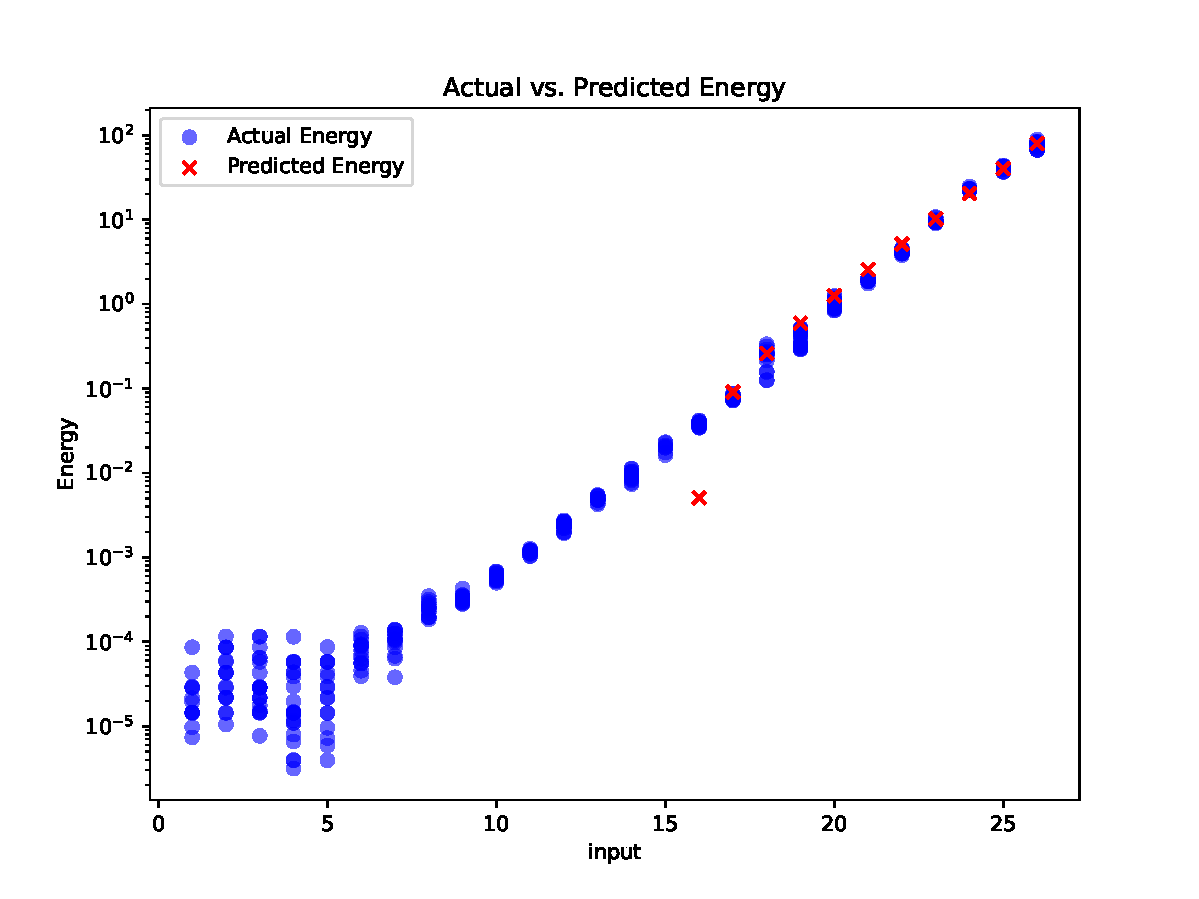
\includegraphics[width = .7 \textwidth]{figures/createTree_plot.pdf}
  \caption{Energy for method \texttt{createTree}}
  \label{fig:createTree_plot}
\end{figure}

\begin{figure}[htbp]
  \centering
  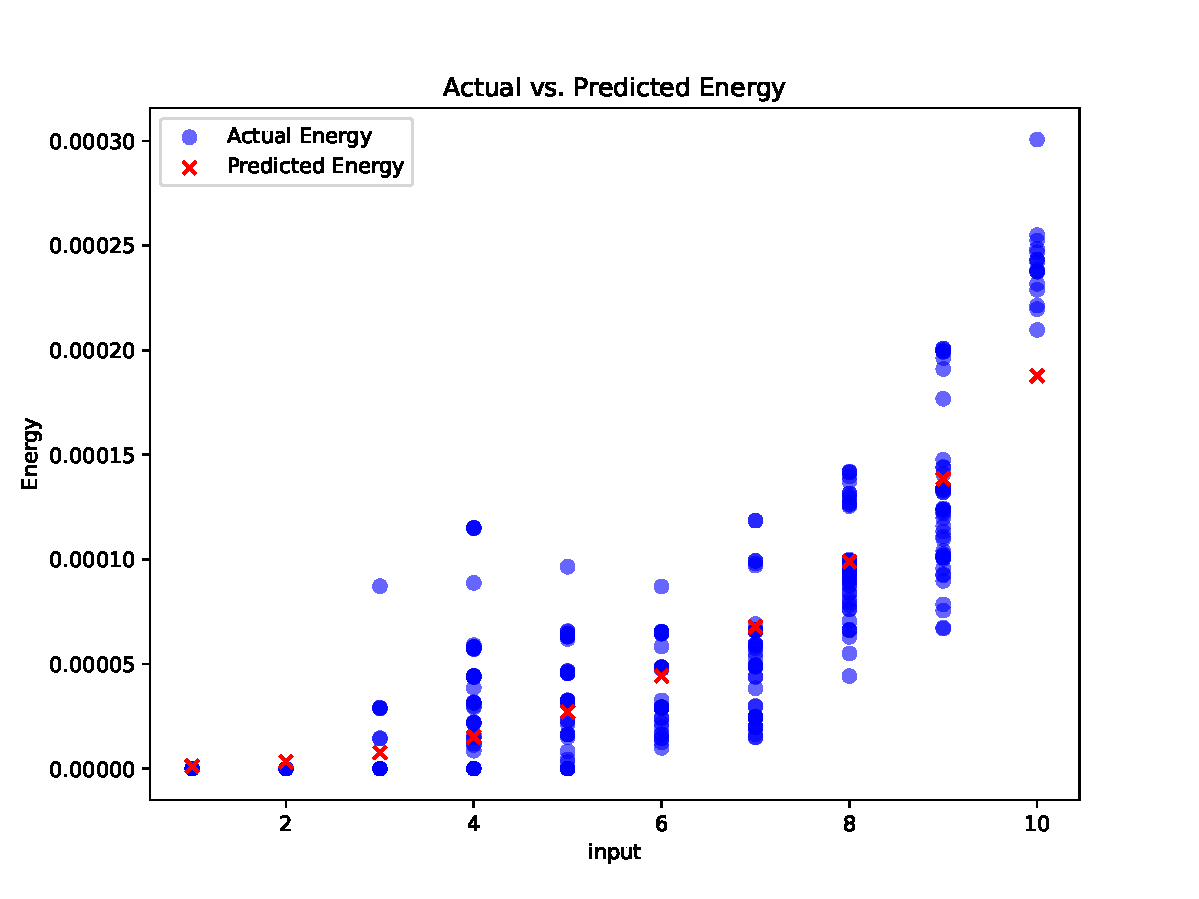
\includegraphics[width = .7 \textwidth]{figures/checkTree_plot.pdf}
  \caption{Energy for method \texttt{checkTree}}
  \label{fig:checkTree_plot}
\end{figure}

\begin{figure}[htbp]
  \centering
  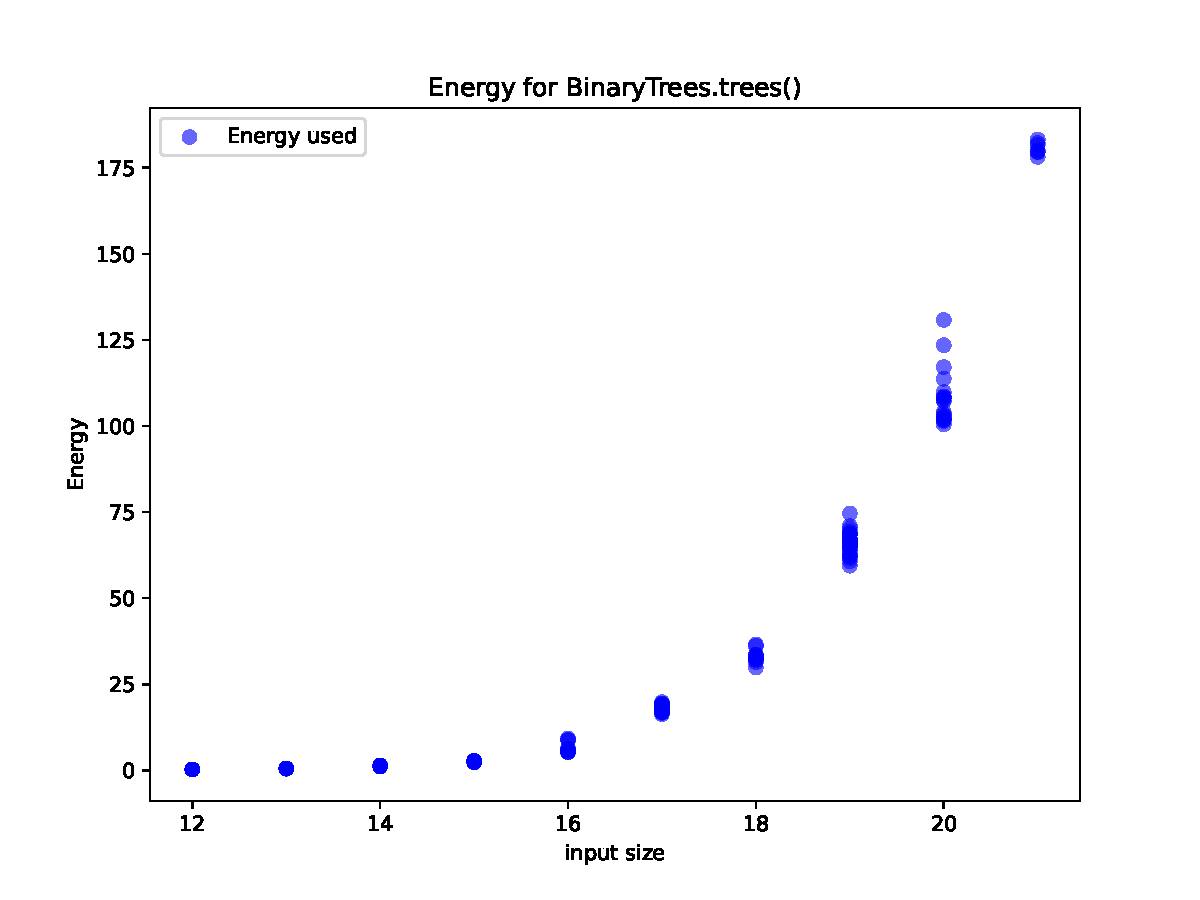
\includegraphics[width = .7 \textwidth]{figures/trees_plot.pdf}
  \caption{Energy for method \texttt{trees}}
  \label{fig:trees_plot}
\end{figure}


{\color{blue}
  Another experiment was conducted using a test case considered more realistic than the others. The program was selected from the Computer Language Benchmarks Game, which provides algorithmic benchmarks designed to test language performance on tasks that are representative of certain real-world computational workloads~\cite{benchmarksGameJava}.

The program selected was the \texttt{}{BinaryTrees} (Java naot #3), which are computational intensive task. It contains three core methods, described as follows:


\begin{itemize}
  \item \textbf{createTree:} Recursively builds a binary tree of the given depth. At each level, creates a node with two children (left and right), until depth equals zero. The result is a complete binary tree with \(2^{\text{depth}} - 1\) nodes.
 
  \item \textbf{checkTree:} Recursively traverses the tree and counts the number of nodes. For leaf nodes, it returns \texttt{1}. For internal nodes, it returns the sum of the recursive calls on the left and right subtrees plus one: $1 + \text{check(left)} + \text{check(right)}$.
  
  \item \textbf{trees:} Performs the core part of the benchmark by creating and checking many binary trees of varying depths and keeping one long-lived tree in memory to simulate memory pressure.
\end{itemize}
}

{\color{blue}
  The Figures~\ref{fig:createTree_plot},~\ref{fig:checkTree_plot}, and~\ref{fig:trees_plot} show the energy of each method, for different input sizes, for every program generated and analyzed by the framework. It is possible to see that the methods have an exponential tendency with the increase of the input, which is expected from binary trees operations. It is also noticeable that the Figure~\ref{fig:checkTree_plot} has a lower curve and input, this was due to the fact that the method required that a tree was created before the method could be run, which would take more time, subsequently, the maximum input for this method was lower. 


From how the program is implemented on the website it needs some small adjustments in order to work with our framework. First, the program does not have a constructor for the class \texttt{TreeNode} which does not allow the program generator to populate the programs correctly, as the program on the website uses a custom method that create the nodes. Without this change, the methods that required \texttt{TreeNode} as input would be simply receiving an empty Object, as the constructor was also empty, making their generation useless as every program would be the same.
With that said, the only adjustments made to the class were, a new private empty constructor, that can only be accessed inside the class, so the generator does not detect it and use it, as the generator always tries to use the smallest one available, so it is important that the empty constructor is private. And it was added a new constructor, this one public, that had the same logic as the method that created the nodes. Now the methods that use \texttt{TreeNode} can be generated as the constructor can call the public constructor that has the similar behavior of the \texttt{createTree(int)} method. These changes do not impact how the program, or methods behave and only helps the program generation.

After that the data was collected and the models for each method used in the program was trained.
}

\begin{table}[htbp]
  \centering
  \footnotesize
  \setlength{\tabcolsep}{10pt} % increase column separation
  \makebox[\textwidth][c]{%
    \begin{tabular}{@{}p{5.3cm}@{\hspace{2.5em}}c@{\hspace{1em}}c@{\hspace{1em}}c@{\hspace{1em}}c@{}}
      \toprule
      Method & Input Value & Predicted Energy (J) & Actual Energy Range (J) & Prediction Error (\%) \\
      \toprule

      \multirow{3}{*}{\texttt{BinaryTrees.createTree(int)}} 
        & 10 & -0.083 & 3.75e-4 -- 4.60e-4 & 19980 \\
        & 23 & 10.26 & 11.78 -- 12.63 & 15.9 \\
        & 26 & 79.90 & 77.29 -- 80.63 & 1.2 \\
      \midrule

      \multirow{3}{*}{\texttt{BinaryTrees.checkTree(TreeNode)}}
        & 10 & 1.88e-4 & 1.64e-4 -- 1.75e-4 & 10.9 \\
        & 23 & 2.19e-3 & 1.37 -- 1.56 & 99.85 \\
        & 26 & 3.15e-3 & 11.72 -- 13.29 & 99.97 \\
      \midrule

      \multirow{3}{*}{\texttt{BinaryTrees.trees(int)}}
        & 10 & -3.42 & 0.041 -- 0.045 & 8053 \\
        & 23 & 517.89 & 713 -- 800 & 31.59 \\
        & 26 & 2429 & 6260 -- 7111 & 63.66 \\
      \midrule

      \multirow{3}{*}{\shortstack[l]{\texttt{BinaryTrees.checkTree(TreeNode)} +\\\texttt{createTree(int)} +\\\texttt{trees(int)}}}
        & 10 & -3.49 & 4.59e-2 -- 4.77e-2 & 7578 \\
        & 23 & 528.15 & 796 -- 806 & 34.08 \\
        & 26 & 2509 & 7062 -- 7350 & 65.18 \\
      \bottomrule
    \end{tabular}%
  }
  \caption{Comparison of actual and predicted energy consumption for BinaryTrees program}
  \label{tab:energy_comparison_bin_trees}
\end{table}



%\begin{table}[htbp]
%  \centering
%  \footnotesize
%  \setlength{\tabcolsep}{10pt}
%  \makebox[\textwidth][c]{%
%    \begin{tabular}{@{}p{5.3cm}@{\hspace{2em}}c@{\hspace{1em}}c@{\hspace{1em}}c@{\hspace{1em}}c@{}}
%      \toprule
%      Method & Input Value (\%) & Predicted Energy Simple Model (J) & Predicted Energy Best Model (J) & Actual Energy Range (J) & Prediction Error Simple Model (\%) & Prediction Error Best Model (\%) \\
%      \toprule
%
%      \multirow{3}{=}{\texttt{BinaryTrees.createTree(int)}} 
%        & 10 & -0.083 & 5.63e-04 & 3.75e-4 -- 4.60e-4 & 19980 & 34.97 \\
%        & 23 & 10.26 & 9.42 & 11.78 -- 12.63 & 15.9 & 22.83 \\
%        & 26 & 79.90 & 80.11 & 77.29 -- 80.63 & 1.2 & 1.45 \\
%      \midrule
%
%      \multirow{3}{=}{\texttt{BinaryTrees.checkTree(TreeNode)}}
%        & 10 & 1.88e-4 & 2.28e-04 & 1.64e-4 -- 1.75e-4 & 10.9 & 34.4 \\
%        & 23 & 2.19e-3 & 2.43e-03 & 1.37 -- 1.56 & 99.85  & 99.83\\
%        & 26 & 3.15e-3 & 3.53e-03 & 11.72 -- 13.29 & 99.97 & 99.97\\
%      \midrule
%
%      \multirow{3}{=}{\texttt{BinaryTrees.trees(int)}}
%        & 10 & -3.42 & 1.69 & 0.041 -- 0.045 & 8053 & 3833 \\
%        & 23 & 517.89 & 798 & 713 -- 800 & 31.59 & 5.49\\
%        & 26 & 2429 & 39754 & 6260 -- 7111 & 63.66 & 494.63 \\
%      \midrule
%
%      \multirow{3}{=}{\parbox{5.3cm}{\centering\texttt{BinaryTrees.checkTree(TreeNode) +\\ createTree(int) + trees(int)}}}
%        & 10 & -3.49 & 4.59e-2 -- 4.77e-2 & 7578 \\
%        & 23 & 528.15 & 796 -- 806 & 34.08 \\
%        & 26 & 2509 & 7062 -- 7350 & 65.18 \\
%      \bottomrule
%    \end{tabular}%
%  }
%  \caption{Comparison of actual and predicted energy consumption for BinaryTrees program}
%  \label{tab:energy_comparison_bin_trees}
%\end{table}



{\color{blue}
The results are detailed in the Table~\ref{tab:energy_comparison_bin_trees}. 

It is noticeable that the values predicted are not the most accurate, for some inputs it has good accuracy, for example, the method \texttt{createTree} has good accuracy for the input \texttt{26}. For other methods, like \texttt{trees} it does not. Again as the previous experiment, the tool is not very accurate in terms of absolute values, and in this case for methods that change their energy considerably with minimum increase in the input, the models have a harder time to predict. The tool demonstrates good relative energy prediction, as input values increase, the predicted energy consumption also increases, and it decreases correspondingly when the inputs are reduced.

To achieve better results with the \texttt{BinaryTrees} methods it could be possible to improve the feature's selection by incorporating characteristics that better capture the program complexity and increase the maximum input available for each program generated in order to better represent the high-energy regions of execution.

However, this experiment objective's was not focused only on achieving the highest accuracy possible. It was also made to prove that it is possible to use the framework to test more interesting and complex cases. And it was proven that with minimal changes, it was possible to mass generate programs, collect data and train models, for the \texttt{BinaryTrees} program. While it may not work universally for all programs, since creating a framework general enough to handle every case is challenging, this experiment demonstrates that analyzing custom programs is possible.
}




\section{Limitations and Challenges} \label{sec:limitations_and_challenges}

During program generation, most of the tested collections focused on List, Set, and Map. However, programs were also generated for another collection category, the Math collection. This introduced an issue. The computations in these programs were extremely fast, completing too quickly for PowerJoular to measure any meaningful energy consumption. As a result, all energy readings for the Math collection programs were reported as 0J.
The problem was the array sizes used to hold the method parameters. While the three predefined array sizes worked well for List, Set, and Map collections, they were too small for the Math collection. The smaller input sizes caused the Math computations to execute very fast, not giving PowerJoular enough time to capture energy usage.
This highlights a challenge in energy profiling: some collections, especially those involving lightweight or highly optimized operations like Math functions, may be difficult to measure accurately. One possible solution would be to determine array sizes during program generation, large enough to ensure that each program runs for at least one second, giving PowerJoular sufficient time to measure energy consumption. However, implementing this would significantly increase the time required for program generation, as it would involve exploring many more combinations of input sizes to find suitable configurations.


Another important factor is that the tool is not able to predict energy when threads are involved, as the programs generated only used a single thread, subsequently the models will not have that factor into account. This limitation exists because measuring and modeling the energy usage of multithreaded programs is particularly challenging due to factors like concurrent execution, thread scheduling, and synchronization overhead. However, threading can deeply impact the energy usage of a program, as a program execution stop being strictly linear, and can have multiple simultaneous computations, potentially increasing the code energy consumption.

{\color{blue}
  A limitation detected during the experimentation of analyzing an external program, was how the inputs on some programs are defined. For example, a program can have a method that receives a String, however, when inside the method it decides to convert the String to int and use it as an Integer, making it so a method that actually uses Integers and not Strings. Although it is easily noticeable by human eye, the program generator cannot understand this kind of context changes as easy, and it would start generating inputs for Strings instead of Integers, which would fail in the program generation. A good example of this usage is when the main function is called and receives the arguments in the \texttt{String[]} and then it uses its values in different variables.
}




%In the start of the project, some tools were tested in order to see how to get the energy profiles for later use. The tools tested were PowerJoular, Powertop, Perf and JoularJx.
%
%Perf is a Linux tool primarily designed for analyzing application performance characteristics rather than precise energy measurement. While it can provide some energy-related metrics, its measurements tend to be imprecise. In this context, Perf was used mainly to get a rough idea of energy consumption and to serve as an alternative when more accurate tools were unavailable.
%
%Powertop was also tested, but it could only perform energy measurements on laptops, as it relies on battery drain data to calculate energy consumption. Since this approach doesn't align with our specific requirements, we considered Powertop as a last-resort option.
%
%JoularJx is an energy measurement tool capable of measuring the consumption of Java programs and its methods. However, it is not as precise as other tools as it requires to measure the entire start of the JVM and whole functions instead of small code blocks.
%
%As described in the \ref{sec:background_energy}, PowerJoular is the best option. As a command line program it can be easily adapted to measure any program or code snippet in most languages. So it was combined with the framework experiment-runner, that facilitates the process.
%
%Initially, JoularJx and the experiment-runner using PowerJoular were used to explore their capabilities and familiarize with the tools. A sample Fibonacci program written in Java and C was used as a test case. However, the energy measurements provided by the two tools differed, and the experiment runner occasionally encountered errors. Later, it was determined that these problems were due to incorrect use of the framework. However, it was still decided the best approach was to make a new orchestrator similar to the Experiment-Runner, but simpler and specifically focused on measuring process energy consumption using PowerJoular. A Java-based orchestrator was initially developed because the Fibonacci implementation was also in Java. However, when tested, the energy measurement results differed significantly from those of the experiment runner, even though the main difference was the programming language (Java vs. Python).
%
%To further analyze these inconsistencies, another orchestrator was developed in Python. This allowed for a closer examination of the differences in energy measurements and a deeper understanding of the behavior of the tools.
%
%Using the process explained on \ref{chapter:approach} it was noticeable that the Java orchestrator was getting significantly more energy consumption than the Python one, which is not very logical, since they both target the same program. So, to try and check which one was having problems, two more orchestrators were implemented, one in C and another in bash.
%
%After running the tests again it was possible to see that the Python orchestrator was getting values way more different from the other three orchestrators as show in Figure \ref{fig:4_orchs_comparison}.
%The figure contains 100 runs of the Fibonacci recursive program written in Java and order by the less energy to the highest energy. And it shows the energy reads for the four different orchestrators used. The labels contain the average energy values and its standard deviation.
%
%Further analysis of the orchestrators revealed a notable difference in behavior. When the Python orchestrator was running, both the parent and child processes consumed CPU resources. In contrast, the other orchestrators (Java, C, and Bash) showed CPU usage only in the child process. This disparity may explain why PowerJoular reported lower energy consumption for the Python orchestrator. Since the CPU load was shared between the parent and child processes, PowerJoular, which measures energy only for the child process (the target Fibonacci program), captured less total energy usage.
%Since the experiment runner included an example demonstrating how to use the framework with PowerJoular, the authors were made aware of this potential conflict when launching PowerJoular from Python.
%
%\begin{figure}%[h]
%  \centering
%  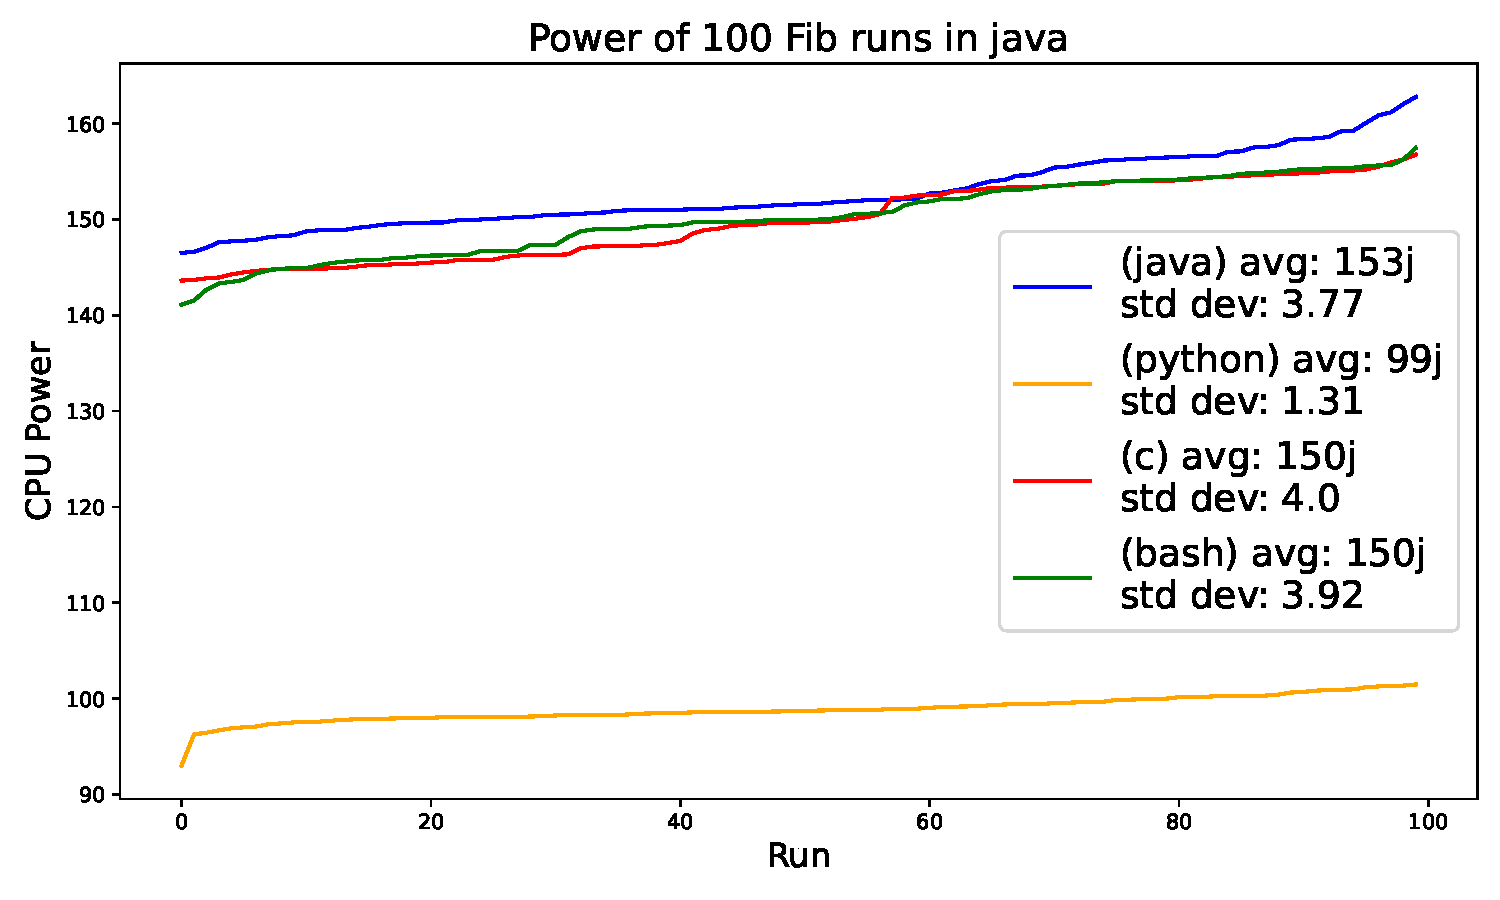
\includegraphics[width = 0.5 \textwidth]{figures/4_orchestrators_comparison.pdf}
%  \caption{orchestrators comparison}
%  \label{fig:4_orchs_comparison}
%\end{figure}

% Conclusao
% Conclusao

\chapter{Conclusion}

The techniques and tools in past and recent research have been studied, and this work improves on those different research and tools, by providing an easy-to-use tool that is also easy accessible and provides energy estimations.
For now, the tool to perform the energy profiling as been selected, (PowerJoular) and a process to create the profiles has been made. This process, as explained in section \ref{sec:work_step1_energy_profiling}, allows targeting specific parts of programs, or the entire program, measure the energy consumption and extract important features. The selection of the tools had some setbacks. When testing PowerJoular it was noticed that it didn't work correctly when using python as an orchestrator, obtaining different measurements than the other orchestrators, (Java, C, Bash), as explained in section \ref{sec:preliminaryresults}. Other than that, the tool worked fine, and it's capable of completing its task of energy profiling. The next step is to start the development of the energy inference function, by collecting the required data. When completed, it is expected that the tool can raise energy awareness among developers, and help facilitate the process of making energy efficient code.


%future work
\chapter{Future Work}

Building on the progress made so far, additional energy profiles must be created to develop a robust energy inference function. This task involves collecting profiles from different machines and gathering enough data to effectively train the machine learning model. The static analysis tool will be implemented and used to provide important code, specifically, certain features that will feed into the model.

After that the efforts will be on developing the actual energy inference function. This task is expected to be the most time-consuming, as it is crucial to the tool functioning. It is most likely that this task overlaps the energy profiling task as more profiles might need to be collected. The task will start by implementing the ML algorithms described in \ref{sec:background_machine_learning}, test their accuracy and improving it by tuning the energy profiles for many possible cases.

When the function is completed, it will be tested against other tools to ensure its quality. The extension will then be built and tested in IDEs.
While developing the function and the extension, the writing of the thesis will also be done in parallel documenting every information.

\begin{figure*}%[h]
  \centering
  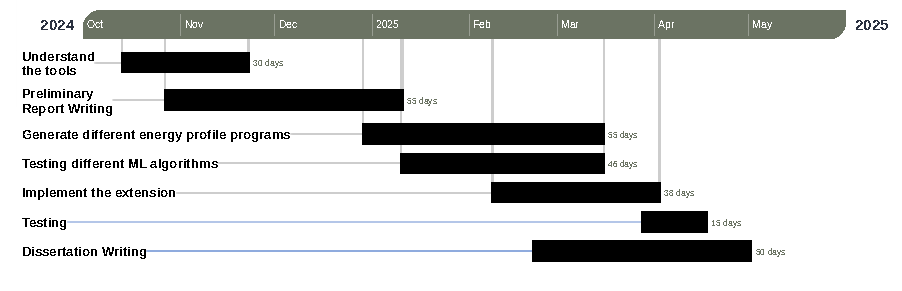
\includegraphics[width = 1 \textwidth]{figures/gantt_diagram.pdf}
  \caption{Work Plan}
  \label{fig:gantt_diagram}
\end{figure*}


The work plan is illustrated more clearly in Figure \ref{fig:gantt_diagram}, which provides a visual representation of the described tasks. While the dates shown in the figure may not precisely align with the actual timeline, the sequence of tasks remains accurate.

% Fim do conteudo
% ----------------------------------------------------------------------

% Glossario

%\LIMPA

%
% Para actualizar o glossario, e' preciso correr o script ./fazindice
% e voltar a gerar o PDF
%
\glossary{name=CPU,description=Central Processor Unit}
\glossary{name=MMU,description=Memory Management Unit}

%\renewcommand{\glossaryname}{Abreviaturas}
%\setglossary{glodelim={\noexpand}}
%\setglossary{glsnumformat=ignore}
\printglossary
\addcontentsline {toc} {chapter} {\glossaryname}

% Bibliografia

%\LIMPA
\nocite{*}
\bibliographystyle{unsrt}
\bibliography{bibliography}
\addcontentsline {toc} {chapter} {\bibname}

% Indice remissivo
%\LIMPA
\printindex
\addcontentsline {toc} {chapter} {\indexname}

% Inicio apendices
\appendix



\end{document}
